% Working-paper version of the repository manuscript.
% Layout and fonts follow the supplied working-paper template.
% Manuscript text, mathematics, references, and numbering are retained.
\documentclass[11pt,a4paper,fleqn]{article}
\usepackage[margin=1.2in]{geometry}
\usepackage{setspace}
\usepackage{mathpazo}
\usepackage[T1]{fontenc}
\usepackage[utf8]{inputenc}
\usepackage{microtype}
\usepackage{amsmath,amsthm,amssymb,mathtools,bm}
\usepackage{booktabs,array,longtable,enumitem}
\usepackage{caption}
\usepackage[dvipsnames]{xcolor}
\usepackage[authoryear,longnamesfirst]{natbib}
\usepackage{xurl}
\usepackage[colorlinks=true,linkcolor=blue!45!black,citecolor=blue!45!black,urlcolor=blue!45!black]{hyperref}
\usepackage{tikz,pgfplots}
\pgfplotsset{compat=1.18}
\usetikzlibrary{arrows.meta,positioning,calc}
\usepackage{float,needspace}
\usepackage[nameinlink,capitalise,noabbrev]{cleveref}

\onehalfspacing
\setlength{\parskip}{0.25em}
\setlength{\parindent}{1.5em}
\setlength{\emergencystretch}{2em}
\setcitestyle{citesep={,}}
\interfootnotelinepenalty=10000

\definecolor{normalblue}{HTML}{0072B2}
\definecolor{normalorange}{HTML}{D55E00}
\definecolor{normalgreen}{HTML}{009E73}
\definecolor{nodegray}{HTML}{F2F4F7}
\definecolor{clearinggreen}{HTML}{D8F0E7}

\hypersetup{
  pdftitle={Buyer-Specific Payments Separate Equilibrium Convexity from Posted-Price Integrability},
  pdfauthor={Zhongji Wei},
  pdfsubject={Working paper},
  pdfkeywords={buyer-specific payments, Walrasian equilibrium, gross substitutes, imperfectly transferable utility, convex potential, price adjustment}
}

\theoremstyle{plain}
\newtheorem{theorem}{Theorem}
\newtheorem{proposition}{Proposition}
\newtheorem{corollary}{Corollary}
\newtheorem{lemma}{Lemma}[section]
\theoremstyle{definition}
\newtheorem{example}{Example}
\newtheorem{definition}{Definition}

% Retain the original manuscript's appendix and equation identifiers.
\AddToHook{cmd/appendix/after}{%
  \setcounter{equation}{0}%
  \counterwithin*{equation}{section}%
  \renewcommand{\thesection}{\appendixname~\Alph{section}}%
  \renewcommand{\theequation}{\Alph{section}.\arabic{equation}}%
  \renewcommand{\thefigure}{\Alph{section}.\arabic{figure}}%
  \renewcommand{\thetable}{\Alph{section}.\arabic{table}}%
}

\newcommand{\R}{\mathbb{R}}
\newcommand{\Z}{\mathbb{Z}}
\newcommand{\co}{\operatorname{co}}
\newcommand{\argmin}{\operatorname*{arg\,min}}
\newcommand{\argmax}{\operatorname*{arg\,max}}
\newcommand{\diag}{\operatorname{diag}}
\newcommand{\relint}{\operatorname{relint}}
\newcommand{\Ecal}{\mathcal{E}}
\newcommand{\Dcal}{\mathcal{D}}
\newcommand{\Pcal}{\mathcal{P}}
\newcommand{\Xcal}{\mathcal{X}}
\newcommand{\one}{\mathbf{1}}
\newcommand{\zero}{\mathbf{0}}
\newcommand{\eps}{\varepsilon}


\begin{document}

\title{\bfseries Buyer-Specific Payments Separate Equilibrium Convexity from Posted-Price Integrability}

\author{Zhongji Wei\thanks{Department of Economics and Business, Universitat Pompeu Fabra. Email: \href{mailto:zhongji.wei@upf.edu}{zhongji.wei@upf.edu}}}
\date{}
\maketitle

\begin{abstract}
Transferable-utility substitutes markets have convex equilibrium-price sets and a convex excess-supply potential. We classify when both survive buyer-specific payments on the full nonnegative price domain. For smooth schedules, universal equilibrium convexity holds exactly for affine rank-one and common log-affine schedules. With three or more buyers and goods, affine rank one is also the exact smooth boundary of posted-price integrability: previous work gives sufficiency, and we prove necessity through a three-good log-affine market that fails a cycle-compatibility test. A three-buyer, two-good linear market admits no polyhedral posted-price potential in any neighborhood of an interior price below its minimum equilibrium price, resolving a previously posed lower-box existence question. The same market admits no convex posted-price potential along the realized ascending-auction path, where the direction resets. For continuous, finitely piecewise-linear schedules, both universal boundaries coincide at affine rank one. General separable payments retain a convex effective-price objective.
\end{abstract}

\noindent\textbf{Keywords.} buyer-specific payments; Walrasian equilibrium; gross substitutes; imperfectly transferable utility; convex potential; price adjustment
\thispagestyle{plain}

\noindent\textbf{JEL classification:} D51, D47, C61.

\clearpage

\section{Introduction}\label{sec:introduction}

Convex potentials organize transferable-utility substitutes markets both at and away from equilibrium: the equilibrium-price set is convex, so averaging two equilibrium prices preserves equilibrium, and excess supply is the subgradient of a convex Walrasian objective, so price adjustment can be studied as convex optimization. We ask when these two properties survive once payments cease to equal posted prices.

Buyer-specific schedules arise when platforms apply commissions, discounts, taxes, or contract-specific transfer rules.\footnote{Within the present price-only model, stylized examples include good-specific category commissions, buyer-specific ad valorem wedges, and continuous price-bracket schedules with changing marginal rates. Volume tiers or rebates that depend on cumulative transactions lie outside the model.} Let $q_{ij}(p_j)$ be buyer $i$'s payment for one unit of good $j$ at posted price $p_j$; the schedules may vary across both buyers and goods. When separability supplies a buyer-common effective-price coordinate, the distinction from posted prices is substantive: mechanisms publicly quote and update $p$, equilibrium convexity concerns averages in $p$, and effective-price descent pulls back through an inverse Jacobian. A single posted-price potential asks more: the current posted-price vector alone determines one convex objective and one subgradient geometry, without additional regime or history variables.

Our first result classifies universal equilibrium convexity for smooth schedules on the full nonnegative price domain. A family passes every two-buyer, two-good unit-demand test with one unit of each good, and equivalently every induced substitutes-market test, exactly when it has one of two forms:
\[
q_{ij}(p_j)=\alpha_i\beta_jp_j
\qquad\text{or}\qquad
q_{ij}(p_j)=\alpha_i\log(1+\beta_jp_j).
\]
Here universal means across every substitutes market induced by every buyer--good restriction of the schedule family, and failure of the universal test need not imply failure in a particular market. The log-affine exception reflects the special geometry of substitutes equilibrium prices: a common logarithmic coordinate turns their coordinate-difference bounds into affine inequalities in shifted posted prices \citep{murota2003,moriguchimurota2023}. That exception is what separates the two properties, since without it the two classifications would coincide, and \Cref{cor:piecewise} shows it disappears once schedules are continuous and finitely piecewise linear, the class to which bracket commissions and tiered taxes belong.

The second property is stricter because a posted-price potential must integrate the excess-supply correspondence away from equilibrium, even after allowing an arbitrary positive, good-specific, and price-dependent rescaling. We require one finite convex function on the entire nonnegative price domain and impose the diagonal subgradient identity at every strictly positive price. \citet{okisato2026} establish affine rank-one sufficiency through a scaled Lyapunov function. We prove necessity: in a three-buyer, three-good log-affine market, the relative scales fixed at three switching-facet intersections are inconsistent around a cycle. Affine rank one is therefore the exact smooth boundary for universal existence of a posted-price diagonal potential.

We then ask whether two auction-motivated weakenings restore existence: imposing the identity only below the minimum equilibrium price, where \citet{okisato2026} pose an open problem, or only along a realized path of their ascending auction, with the direction map tied to the direction their Local Stability Condition selects. A three-buyer, two-good linear market (\Cref{ex:two-good}) defeats both. Below the minimum equilibrium price, two transverse switches force a two-dimensional subdifferential while every diagonally scaled excess-supply set is a segment; along the realized path, a forced direction reset and closedness of convex subdifferentials prevent one potential from covering both regimes.

For continuous finitely piecewise-linear schedules, affine rank one is necessary and sufficient for both universal global properties. A genuine kink therefore removes the universal guarantee of one posted-price potential. More generally, Proposition~\ref{prop:effective} identifies the integrated effective-price coordinate in which the Walrasian objective remains convex.

The equilibrium classification comes from vanishing local two-by-two slope minors, which force marginal payments to factor into buyer and good components, after which straight indifference sets leave only affine and common log-affine coordinates. The potential result uses a different obstruction: flat clearing facets fix subgradient endpoints, and three ridge comparisons transport them around a cycle whose scale ratios are inconsistent. In the two-good market, transverse switching and a forced direction reset become a dimension contradiction and a closed-graph contradiction.

Our analysis builds on the gross-substitutes and assignment traditions \citep{shapleyshubik1971,kelsocrawford1982,bikhchandanimamer1997,danilovkoshevoymurota2001,murota2003,baldwinklemperer2019}, and in particular on the Walrasian price structure under gross substitutes developed by \citet{gulstacchetti1999} and \citet{milgromstrulovici2009}. Matching with contracts provides a broader market-design lineage for heterogeneous contractual terms \citep{hatfieldmilgrom2005}, while non-quasilinear auction design studies other consequences of nonlinear payment utility \citep{baisa2017}. Work on imperfect transferability studies existence, lattice structure, comparative statics, and design under broader primitives \citep{demangegale1985,alkan1989,alkan1992,galichonkominersweber2019,baldwinjagadeesanklempererteytelboym2023,fleineretal2019,schlegel2022,galichonweber2024}. We complement that literature by fixing buyer-specific posted-price schedules and classifying the restrictions that recover Euclidean equilibrium convexity and convex integration in posted-price coordinates.

Convex potentials also underlie ascending auctions and continuous price adjustment \citep{gulstacchetti2000,ausubel2006,milgromstrulovici2009,murotaetal2016,paesleme2017}. \citet{cheungcoledevanur2020} derive Bregman updates when a convex potential already exists in posted prices and has excess supply as its gradient, whereas our effective-price result obtains a convex objective only after a nonlinear effective-price change whose pullback need not be posted-price convex. \citet{bedardgoeree2025} study conservative-correspondence integrability in quasilinear indivisible-goods economies, while we classify buyer-specific payment schedules and compare posted-price integrability with equilibrium convexity \citep[see also][]{rockafellar1966,rochet1987,kushnirlokutsievskiy2021}. \citet{balkanskienfaenza2024} propose t\^atonnement procedures for imperfectly transferable assignment games. Closest to the adjustment question, \citet{okisato2026} give a finite ascending auction for strong-substitutes markets with heterogeneous piecewise-linear payments, driven by a direction that is recomputed at each change of the over-demanded set. Our converse and the two local obstructions separate such direction-recomputing auctions from a single integrating potential in posted prices.

\Cref{sec:model} states the model and the main results; \Cref{sec:geometry} proves the equilibrium classification; \Cref{sec:holonomy} proves \Cref{thm:potential} and \Cref{thm:lower-path}; and \Cref{sec:effective} develops the effective-price objective and its posted-price pullback. The appendices collect supporting proofs, discrete-convex inputs, and exact checks.

\Needspace{12\baselineskip}
\section{Model and main results}\label{sec:model}

\subsection{Environment, demand, and equilibrium}\label{subsec:environment}

There are $n$ buyers $N=\{1,\ldots,n\}$ and $m$ indivisible goods $M=\{1,\ldots,m\}$. Supply is $s=(s_j)_{j\in M}\in\Z_+^M$. Buyer $i$ chooses a bundle from a finite set $\Xcal_i\subset\Z_+^M$ and has valuation $v_i:\Xcal_i\to\R$, normalized so that $0\in\Xcal_i$ and $v_i(0)=0$. Throughout, $e_j$ denotes the $j$th unit vector, $\one$ the all-ones vector of the relevant dimension, and $\co$ the convex hull.

At posted prices $p\in\R_+^M$, buyer $i$ pays $q_{ij}(p_j)$ per unit of good $j$ and demands
\begin{equation}\label{eq:demand}
D_i(p)=\argmax_{x\in\Xcal_i}
\left\{v_i(x)-\sum_{j\in M}q_{ij}(p_j)x_j\right\}.
\end{equation}
Each payment function $q_{ij}:\R_+\to\R_+$ satisfies $q_{ij}(0)=0$ and is strictly increasing. The smooth results impose $q_{ij}\in C^1$ and $q'_{ij}>0$. The piecewise-linear results impose continuity, strict monotonicity, and finitely many linear pieces.

A unit-demand buyer has $\Xcal_i=\{0\}\cup\{e_j:j\in M\}$. Extend each valuation to $\Z^M$ by setting $\widetilde v_i(x)=v_i(x)$ on $\Xcal_i$ and $\widetilde v_i(x)=-\infty$ elsewhere. The substitutes class consists of valuations whose extensions are $M^\natural$-concave. This condition is also called strong substitutes on multi-unit domains and agrees with gross substitutes in the binary domain; every unit-demand valuation belongs to this class. Positive rescaling preserves it \citep{murota2003,murota2016,paesleme2017}.

A Walrasian equilibrium is a price vector $p$ and choices $x_i\in D_i(p)$ satisfying $\sum_i x_i=s$. Write $\Ecal(v,q,s)$ for the equilibrium-price set. For nonempty sets $I\subseteq N$ and $J\subseteq M$, the corresponding \emph{buyer--good restriction} keeps the schedules $(q_{ij})_{i\in I,j\in J}$. After fixing these schedules, an induced market may choose any finite bundle sets and substitutes valuations for the buyers in $I$, together with any supply $s\in\Z_+^J$, subject to the preceding assumptions. All universal statements below quantify over these restricted markets.

For any collection $a=(a_i)_{i\in N}$ with $a_i\in\R^M$, write $D_i[a_i]=\argmax_{x\in\Xcal_i}\{v_i(x)-a_i\cdot x\}$. Thus $D_i(p)=D_i[(q_{ij}(p_j))_{j\in M}]$.

For subdifferential statements, define the convexified excess-supply correspondence
\begin{equation}\label{eq:Z}
Z(p)=s-\sum_{i\in N}\co D_i(p),
\end{equation}
where the sum is a Minkowski sum. At a tie, $\co D_i(p)$ permits fractional mixtures of demanded bundles. Under $M^\natural$-concave valuations, convexified clearing is exact: $0\in Z(p)$ holds if and only if demanded bundles themselves clear the market (\Cref{lem:convexified-clearing}). \ref{app:walrasian} records this equivalence together with the coordinate-and-difference-bound representation of Walrasian price sets; the local constructions in the proofs verify demand and clearing directly.

\subsection{Equilibrium convexity and posted-price integrability}\label{subsec:two-notions}

The first property concerns only the geometry of equilibrium prices.

\begin{definition}[Equilibrium convexity]\label{def:eq-convexity}
A payment family has \emph{universal equilibrium convexity} if, on every buyer--good restriction, the equilibrium-price set $\Ecal(v,q,s)$ is a Euclidean convex subset of posted-price space for every induced substitutes market for which equilibrium exists.
\end{definition}

The second property asks for one global integrating potential on the economically feasible price domain. Under transferable utility, the classical Walrasian objective has $Z(p)$ as its subdifferential at every $p$. We retain posted prices as the argument of the potential but allow each good's imbalance to be measured in its own positive, price-dependent unit. Throughout, $L$ denotes a candidate posted-price potential and $\widehat L$ the effective-price objective of \Cref{subsec:effective-objective}.

For a finite convex function $L:\R_+^M\to\R$, write
\[
\partial_+L(p)=
\left\{g\in\R^M:
L(p')\ge L(p)+g\cdot(p'-p)
\text{ for every }p'\in\R_+^M
\right\}
\]
for its subdifferential relative to the nonnegative orthant. At every $p\in\R_{++}^M$, this is the ordinary subdifferential on the interior of the domain.

\begin{definition}[Global posted-price diagonal potential]\label{def:potential}
A market admits a \emph{finite convex posted-price diagonal potential} if there are one finite-valued convex function $L:\R_+^M\to\R$ and a map $d:\R_{++}^M\to\R_{++}^M$ such that
\begin{equation}\label{eq:potential-definition}
\partial_+L(p)=\diag(d(p))^{-1}Z(p)
\qquad\text{for every }p\in\R_{++}^M.
\end{equation}
If $L$ can be chosen polyhedral, the market admits a \emph{polyhedral posted-price diagonal potential}. A payment family is \emph{universally posted-price-integrable} if, on every buyer--good restriction, every substitutes market induced by the restricted payment family admits such a pair $(L,d)$.
\end{definition}

Economically, $d_j(p)$ fixes the local unit in which good $j$'s imbalance is measured, and $1/d_j(p)$ is the corresponding adjustment scale. These units may vary arbitrarily with prices but do not mix goods. We therefore classify integrability under the same diagonal rescaling used in the existing sufficiency result and in the lower-box question of \Cref{subsec:path-relaxations}. The word \emph{global} means that one function $L$ serves the whole nonnegative price domain; cell-specific functions replaced at a breakpoint qualify only if they paste into a single convex function satisfying \eqref{eq:potential-definition}. For a fixed $d$, the identity imposes cyclic monotonicity on the rescaled correspondence; here $d$ and $L$ must be found jointly \citep{rockafellar1966}.

Any posted-price diagonal potential has a convex minimizer set. Under the hypotheses of \Cref{lem:convexified-clearing}, it therefore makes the strictly positive equilibrium-price set convex:
\begin{equation}\label{eq:argmin-equilibrium}
\begin{aligned}
\Ecal(v,q,s)\cap\R_{++}^M
&=\{p\in\R_{++}^M:0\in Z(p)\}\\
&=\{p\in\R_{++}^M:0\in\partial_+L(p)\}\\
&=\argmin_{p\in\R_+^M}L(p)\cap\R_{++}^M.
\end{aligned}
\end{equation}
The minimizer set of a convex function is convex, as is its intersection with $\R_{++}^M$. The common log-affine family shows that this implication is strict.

\subsection{Main classifications}\label{subsec:main-results}

The two classifications are nested. Equilibrium geometry permits affine rank-one payments and one common log-affine coordinate; the posted-price diagonal potential permits only the affine branch. The first boundary is already identified by two unit-demand buyers and two unit-supply goods.

\begin{theorem}[Affine--log-affine equilibrium geometry]\label{thm:geometry}
Suppose $|N|,|M|\ge2$, $q_{ij}\in C^1(\R_+)$, $q_{ij}(0)=0$, and $q'_{ij}>0$. The following statements are equivalent.
\begin{enumerate}[label=(\roman*),leftmargin=2.2em]
\item On every two-buyer, two-good restriction, every unit-demand market with one unit of each good has $\Ecal(v,q,s)\cap\R_{++}^2$ convex.
\item There are positive buyer factors $\alpha_i$ and positive good factors $\beta_j$ such that, after the immaterial common rescaling of the $\alpha_i$, either
\begin{align}
q_{ij}(p_j)&=\alpha_i\beta_jp_j, \label{eq:affine-family}\\
\intertext{for all $i,j$, or}
q_{ij}(p_j)&=\alpha_i\log(1+\beta_jp_j) \label{eq:log-family}
\end{align}
for all $i,j$.
\item The payment family is universally equilibrium-convex; every equilibrium-price set is polyhedral.
\end{enumerate}
\end{theorem}

A two-by-two test therefore identifies the universal boundary. Local convexity first forces buyer heterogeneity into one scalar; straight indifference loci then leave only a linear coordinate or a common logarithmic coordinate. The proof follows these two steps and uses \Cref{lem:walrasian-price-polyhedron} for sufficiency. No unboundedness assumption is imposed: schedules are defined on all of $\R_+$, and the proof derives unboundedness of the classified effective-price coordinates.

Both families make every buyer weigh one common cross-good price index against a personal threshold. Under affine rank-one payments the index is the difference in rescaled prices $\beta_jp_j-\beta_kp_k$; under log-affine payments it is the ratio of shifted prices $(1+\beta_jp_j)/(1+\beta_kp_k)$. In either case the prices at which a buyer switches goods form a hyperplane in posted prices, so equilibrium sets are carved out by affine inequalities and averaging preserves them.

Under their Assumption~4.1, which is the affine rank-one family, \citet[Theorem~6.4]{okisato2026} establish sufficiency through a scaled Lyapunov function. The next theorem proves the universal converse and thereby completes the exact boundary.

\begin{theorem}[Exact smooth boundary of posted-price integrability]\label{thm:potential}
Suppose $|N|,|M|\ge3$ and that payments satisfy the smooth assumptions of \Cref{thm:geometry}. The following statements are equivalent.
\begin{enumerate}[label=(\roman*),leftmargin=2.2em]
\item Every unit-demand market on every restriction with at most three buyers and at most three goods admits a finite convex posted-price diagonal potential.
\item There are positive factors $\alpha_i,\beta_j$ such that
\[
q_{ij}(p_j)=\alpha_i\beta_jp_j
\qquad\text{for all }i,j,p_j.
\]
\item The payment family is universally posted-price-integrable.
\end{enumerate}
When these conditions hold, the potential may be chosen polyhedral.
\end{theorem}

The distinction appears off equilibrium. A global diagonal potential commits the auctioneer to one objective whose local units must be compatible across all switching facets. In the three-good log-affine market constructed below, each of three facets fixes the relative scale of two goods, and the three requirements conflict around a cycle. The proof allows any finite convex $L$ on $\R_+^M$ and any positive, possibly discontinuous $d$. Flat-minimizer rigidity fixes one subgradient endpoint on each clearing facet, and facet-to-ridge endpoint transport carries those endpoints to the ridges where the scale ratios conflict.

For finitely piecewise-linear schedules, the nonlinear branch is unavailable and the two boundaries coincide.

\begin{corollary}[Piecewise-linear boundary]\label{cor:piecewise}
Suppose $|N|,|M|\ge2$ and each $q_{ij}:\R_+\to\R_+$ is continuous, strictly increasing, finitely piecewise linear, and satisfies $q_{ij}(0)=0$. The following are equivalent:
\begin{enumerate}[label=(\roman*),leftmargin=2.2em]
\item on every two-buyer, two-good restriction, every unit-demand market with one unit of each good has a convex equilibrium-price set;
\item the payment family is universally equilibrium-convex;
\item the payment family is universally posted-price-integrable;
\item payments are affine rank one: $q_{ij}(p_j)=\alpha_i\beta_jp_j$ for positive factors $\alpha_i,\beta_j$.
\end{enumerate}
Under these equivalent conditions, the potential in (iii) may be chosen polyhedral.
\end{corollary}

In market terms, the corollary speaks to bracket schedules: a commission or tax whose marginal rate changes at a threshold price puts a kink into some payment coordinate, and one such kink already removes both universal guarantees. In the auction of \citet{okisato2026}, a good factor that is piecewise constant in its own price triggers a restart from the current price with a new potential; the corollary shows that no single potential replaces such a restarted family across all markets. \Cref{tab:results-summary} collects the boundaries.

In summary, for smooth families with at least three buyers and three goods,
\[
\begin{aligned}
\{\text{universally posted-price-integrable}\}
&=\{\text{affine rank one}\}\\
&\subsetneq
\{\text{universally equilibrium-convex}\}\\
&=\left\{\substack{\text{affine rank one or}\\
\text{common log-affine}}\right\}.
\end{aligned}
\]

\begin{table}[!t]
\centering
\caption{Exact universal posted-price boundaries.}
\label{tab:results-summary}
\small
\setlength{\tabcolsep}{4pt}
\begin{tabular}{@{}>{\raggedright\arraybackslash}p{0.30\textwidth}>{\raggedright\arraybackslash}p{0.18\textwidth}>{\raggedright\arraybackslash}p{0.23\textwidth}>{\raggedright\arraybackslash}p{0.19\textwidth}@{}}
\toprule
Universal property & Schedule class & Exact boundary & Detecting restriction \\
\midrule
Equilibrium convexity & smooth & affine rank one or common log-affine & two-buyer, two-good \\
Posted-price diagonal potential on $\R_+^M$ & smooth & affine rank one & at most three-by-three \\
Both properties & continuous, finitely piecewise-linear & affine rank one & two-buyer, two-good \\
\bottomrule
\end{tabular}
\end{table}

\Needspace{10\baselineskip}
\subsection{Local obstructions in a linear two-good market}\label{subsec:path-relaxations}

We impose \eqref{eq:potential-definition} either on the order interval below the minimum equilibrium price or on one realized auction path. Both restrictions fail locally, and for a local reason, in the following linear two-good market.

\begin{example}[Three buyers, two goods]\label{ex:two-good}
There are two goods, each in unit supply, so $s=(1,1)$, and three unit-demand buyers. The singleton values and payment schedules are
\begin{equation}\label{eq:path-market}
\begin{array}{c|c|cc}
 i &(v_{i1},v_{i2})&q_{i1}(p_1)&q_{i2}(p_2)\\ \hline
 1&(10,10)&p_1&p_2\\
 2&(10,11)&p_1&2p_2\\
 3&(0,5)&p_1&p_2.
\end{array}
\end{equation}
Every payment is linear in the posted price: buyer 2 pays twice the posted price of good 2, while the other five payments equal the posted price. The matrix of marginal payments has rank two, so the affine rank-one potential-existence result does not apply to this market. The minimum equilibrium price is $\bar p=(5,5)$ (\Cref{lem:path-minimum-equilibrium}). Buyer 1 switches goods on the line $p_1=p_2$ and buyer 2 on the line $p_1=2p_2-1$; the two lines cross transversally at $p^\circ=(1,1)$, where buyer 3 uniquely demands good 2.
\end{example}

Let $\bar p$ be the minimum equilibrium price of a market. \citet{okisato2026} pose as an open problem (their Problem~6.2) whether a polyhedral convex $L:\R_+^M\to\R_+$ and a positive diagonal direction map exist that satisfy the scaled excess-supply identity on the order interval below $\bar p$ together with a directional condition at the minimizers. A \emph{lower-box diagonal potential} is any polyhedral convex $L:\R_+^M\to\R$ with a map $d$ from $\{p\in\R_{++}^M:p\le\bar p\}$ to $\R_{++}^M$ satisfying \eqref{eq:potential-definition} at every strictly positive $p\le\bar p$; this class drops the directional condition and the sign restriction on $L$ and imposes the identity only at strictly positive prices, so it is larger and nonexistence is the stronger statement. The problem is posed for their general framework, their affine rank-one assumption entering their sufficiency result rather than the problem statement, so the market of \Cref{ex:two-good} lies within its scope.\footnote{Throughout we use the convexified correspondence $Z=s-\sum_i\co D_i$ of \eqref{eq:Z}, consistently with the Danskin step in the proof of their sufficiency result.}

The second relaxation imposes the identity only along one realized execution of their ascending auction. For the market of \Cref{ex:two-good}, consider the price path
\begin{equation}\label{eq:realized-auction-path}
(0,0)\longrightarrow(0,1/2)
\xrightarrow{\ (2,1)\ }(1,1)
\xrightarrow{\ (1,1)\ }(5,5).
\end{equation}
Call this path $\Gamma$, and let $a^+(p)$ be its outgoing direction at $p$: $a^+(p)=(2,1)$ at every point of the open segment from $(0,1/2)$ to $p^\circ$, and $a^+(p)=(1,1)$ at $p^\circ$ and on the diagonal segment from $p^\circ$ to $\bar p$, excluding $\bar p$, where the auction stops. A pair $(L,d)$ is a \emph{posted-price potential along $\Gamma$} if $L:\R_+^2\to\R$ is finite and convex, $d:\Gamma\cap\R_{++}^2\to\R_{++}^2$, \eqref{eq:potential-definition} holds at every $p\in\Gamma\cap\R_{++}^2$, and $d(p)$ is a positive multiple of $a^+(p)$ at every such $p$ other than $\bar p$. The last requirement couples $d$ to the auction because, in their problem, $d$ is the direction map of the auction itself. The multiple is unrestricted, so time along $\Gamma$ may be reparameterized freely, while the same $L$ must serve before and after the reset.

The ascending auction raises prices along a direction whose positive support is the inclusion-minimal maximizer $X^*(p)$ of the over-demand function
\[
O(X)=\sum_i\min_{x\in\check D_i(p)}x(X)-s(X),
\]
where $\check D_i(p)$ is the set of inclusion-minimal demanded bundles and $x(X)=\sum_{j\in X}x_j$. The direction satisfies their Local Stability Condition (LSC) if $X^*(p)$ remains the unique minimal maximizer after every sufficiently small move along it. \Cref{lem:forced-path} shows that on this market LSC admits exactly the directions displayed in \eqref{eq:realized-auction-path}.

\begin{theorem}[Local obstructions in a linear two-good market]\label{thm:lower-path}
In the market of \Cref{ex:two-good}, let $p^\circ=(1,1)$ and let $\Gamma$ be the path \eqref{eq:realized-auction-path}.
\begin{enumerate}[label=(\roman*),leftmargin=2.2em]
\item For every neighborhood $U\subseteq\R_{++}^2$ of $p^\circ$, no pair of a polyhedral convex $L:\R_+^2\to\R$ and a map $d:U\to\R_{++}^2$ satisfies \eqref{eq:potential-definition} at every $p\in U$. Since $p^\circ<\bar p$, the market admits no lower-box diagonal potential.
\item Every execution of the ascending auction from the zero price whose update directions satisfy LSC follows $\Gamma$, up to positive reparameterization of each segment, and its direction resets at $p^\circ$. For every $\eps>0$, no finite convex $L:\R_+^2\to\R$ satisfies \eqref{eq:potential-definition} at $p^\circ$ and at every point of the incoming segment of $\Gamma$ within distance $\eps$ of $p^\circ$ with a map $d$ into $\R_{++}^2$ that is a positive multiple of $a^+$ at each of these points. In particular the market admits no posted-price potential along $\Gamma$, and this conclusion uses neither polyhedrality of $L$ nor continuity of $d$.
\end{enumerate}
\end{theorem}

Three of the demand cells meeting at $p^\circ$ force three affinely independent subgradients of a polyhedral $L$, while every diagonal rescaling of the segment $Z(p^\circ)$ is a segment; along $\Gamma$, closedness of the subdifferential graph forbids gluing the incoming and outgoing regimes into one convex $L$. Buyer 2's tie fixes the incoming ray and buyer 1's tie fixes the outgoing ray, so the diagonal scale must change where the two tie sets meet. The obstruction concerns one convex objective in posted prices, and the auction itself remains well defined because it recomputes its direction at the reset. \Cref{subsec:lower-path-proof} gives the proofs.

\subsection{Effective-price objective}\label{subsec:effective-objective}

More general separable payments retain a convex objective after changing coordinates. Suppose
\begin{equation}\label{eq:general-separable}
q_{ij}(p_j)=\alpha_iQ_j(p_j),
\end{equation}
where $\alpha_i>0$ and each $Q_j$ is continuous and strictly increasing with $Q_j(0)=0$. Define effective prices $r=Q(p)$ componentwise, let $\mathcal R_Q=\prod_j Q_j(\R_+)$ be their attainable range, and set
\begin{equation}\label{eq:Lhat}
\widehat L(r)=
\sum_i\max_{x\in\Xcal_i}
\left\{\frac{v_i(x)}{\alpha_i}-r\cdot x\right\}
+s\cdot r.
\end{equation}

\begin{proposition}[Effective-price objective]\label{prop:effective}
Suppose \eqref{eq:general-separable} holds. The effective-price objective $\widehat L$ in \eqref{eq:Lhat} is finite, polyhedral, and convex on $\R^M$. For every $r\in\mathcal R_Q$,
\begin{equation}\label{eq:Lhat-subdiff}
\partial\widehat L(r)
=s-\sum_i\co D_i(Q^{-1}(r));
\end{equation}
if, in addition, each $\widetilde v_i$ is $M^\natural$-concave, then posted-price equilibria satisfy
\begin{equation}\label{eq:effective-minimizers}
\Ecal(v,q,s)=Q^{-1}\!\left(\argmin_{r\in\R^M}\widehat L(r)\cap\mathcal R_Q\right).
\end{equation}
\end{proposition}

\Cref{prop:effective} identifies the coordinate in which the standard Walrasian convex objective remains available for general separable payments; \Cref{sec:effective} gives the proof and the posted-price pullback.

\section{Equilibrium convexity: proof of Theorem~\ref{thm:geometry}}\label{sec:geometry}

\noindent\textit{Proof of \Cref{thm:geometry}.} The implication (iii)$\Rightarrow$(i) is immediate. The proof of (i)$\Rightarrow$(ii) separates local buyer heterogeneity from nonlinear coordinate geometry: a schedule outside the two families misaligns two buyers' comparisons at some price pair, and the proof converts that misalignment into two clearing prices with a nonclearing midpoint.

\subsection{Local rank-one necessity}

Fix buyers $i,k$, goods $j,\ell$, and an interior price pair $(t,u)$.

\begin{proposition}[Local minor obstruction]\label{prop:local-minor}
If
\[
q'_{i\ell}(u)q'_{kj}(t)-q'_{ij}(t)q'_{k\ell}(u)\ne0,
\]
then there are unit-demand valuations and two nearby equilibrium prices whose midpoint is not an equilibrium.
\end{proposition}

\begin{example}[A two-by-two failure]\label{ex:two-by-two}
Let $q_{11}(p)=q_{12}(p)=q_{21}(p)=p$ and $q_{22}(p)=2p$, so the matrix of marginal slopes is
\[
\begin{pmatrix}1&1\\1&2\end{pmatrix}
\]
and has nonzero determinant. Give buyer 1 singleton values $(C,C)$ and buyer 2 values $(C,C+1)$, with $C>3$, and supply one unit of each good. At $p^A=(3/10,3/5)$ the buyers uniquely choose goods 1 and 2; at $p^B=(3/2,7/5)$ they uniquely choose goods 2 and 1. Both prices clear. At their midpoint $(9/10,1)$, both buyers uniquely choose good 1. The equilibrium-price set is therefore nonconvex, and by \eqref{eq:argmin-equilibrium} this market cannot admit the posted-price potential in \Cref{def:potential}.
\end{example}

In the general construction, each buyer's singleton-value difference equals the payment difference at $(t,u)$, with the outside option dominated nearby. A nonzero minor makes the two indifference curves cross transversally, so the inverse function theorem yields nearby clearing prices at which the buyers split the goods in opposite ways. At their midpoint both strictly choose good $j$, so clearing fails. \ref{app:factorization} supplies the local sign construction and first-order expansion.

Hence every local marginal $2\times2$ minor vanishes at positive prices; continuity extends the identity to zero. Positivity and connectedness then imply a global factorization.
\begin{equation}\label{eq:all-minors-zero}
q'_{ij}(t)q'_{k\ell}(u)
=q'_{i\ell}(u)q'_{kj}(t)
\qquad\text{for all }i,k,t,u\text{ and distinct }j,\ell.
\end{equation}

\begin{lemma}[Marginal factorization]\label{lem:smooth-factorization}
Under the standing assumptions of \Cref{thm:geometry} and \eqref{eq:all-minors-zero}, there are constants $\alpha_i>0$ and functions $Q_j\in C^1(\R_+)$ with $Q_j(0)=0$ and $Q'_j>0$ such that
\begin{equation}\label{eq:smooth-factorization}
q_{ij}(p)=\alpha_iQ_j(p)
\qquad\text{for all }i,j,p.
\end{equation}
\end{lemma}

Economically, all buyer heterogeneity is now one scalar, while each good has a common effective-price coordinate. The proof, given in \ref{app:factorization}, fixes a reference buyer $i_0$ and uses an auxiliary good to extend the distinct-good identities to same-good comparisons at different prices. The resulting ratio $q'_{ij}/q'_{i_0j}$ is independent of the good and price. Integration uses $q_{ij}(0)=0$.

\subsection{Straight indifference sets and affine price semigroups}

Under \eqref{eq:smooth-factorization}, divide buyer $i$'s utility by $\alpha_i$. Effective prices are $r_j=Q_j(p_j)$. Consider two identical unit-demand buyers and two unit-supply goods $j,k$. Give both buyers the same effective singleton-value difference $c$. In a neighborhood where the outside option is dominated, the market clears exactly when both buyers are indifferent, namely on
\begin{equation}\label{eq:level-set}
Q_j(p_j)-Q_k(p_k)=c.
\end{equation}
If the equilibrium set is convex, every sufficiently short chord between points of this level set must stay on the level set. A graph that is locally convex as a set must be affine. Therefore, for every feasible $c$, the function $T_{jk,c}(x)=Q_k^{-1}(Q_j(x)-c)$ is affine on each connected component of its domain. Because the domain is an interval and the local affine representations overlap, $T_{jk,c}$ is affine on its entire domain.

These cross-good maps form a price-translation semigroup: increasing effective price by $t$ and then $u$ is the same as increasing it once by $t+u$. Let $R_j=\sup_{x\ge0}Q_j(x)$ and, for $0\le t<R_j$, define
\begin{equation}\label{eq:translation-semigroup}
S_{j,t}(x)=Q_j^{-1}(Q_j(x)+t)
\end{equation}
on the interval where $Q_j(x)+t<R_j$. \ref{app:straight-level} shows that each $S_{j,t}$ is affine on its domain, that its coefficients are continuous in $t$, and that, whenever $t,u,t+u<R_j$, effective-price addition gives on the common domain
\begin{equation}\label{eq:semigroup-identities}
\begin{aligned}
S_{j,t}(x)&=a_j(t)x+b_j(t),
&a_j(t)&>0,
&b_j(t)&=Q_j^{-1}(t)\ge0,\\
S_{j,t+u}&=S_{j,t}\circ S_{j,u},
&a_j(t+u)&=a_j(t)a_j(u),
&b_j(t+u)&=a_j(t)b_j(u)+b_j(t).
\end{aligned}
\end{equation}

The continuous affine-semigroup equations have only a translation branch and an exponential-dilation branch. They also rule out a finite $R_j$: the inverse orbit would have to diverge at a finite effective-price boundary, while either affine-semigroup solution remains finite there. Thus unboundedness is a conclusion rather than an assumption, and inversion yields exactly two possibilities:
\begin{equation}\label{eq:inverse-two-forms}
Q_j(x)=\frac{x}{c_j}
\qquad\text{or}\qquad
Q_j(x)=\frac{1}{\gamma_j}\log\left(1+\frac{x}{c_j}\right).
\end{equation}

Finally, $T_{jk,0}=Q_k^{-1}\circ Q_j$ is affine and fixes zero. Cross-good compatibility therefore rules out mixing the two branches and forces a common $\gamma>0$ in the logarithmic branch. Absorbing $1/\gamma$ into the buyer factors $\alpha_i$ and writing $\beta_j=1/c_j$ gives exactly \eqref{eq:affine-family} or \eqref{eq:log-family}. \ref{app:straight-level} supplies the functional-equation and compatibility details. This proves (i)$\Rightarrow$(ii).

\subsection{Why the log-affine family preserves all equilibrium polyhedra}

The sufficiency argument uses a discrete-convex description of Walrasian price sets, stated as \Cref{lem:walrasian-price-polyhedron} in \ref{app:walrasian}. In effective prices, every nonempty substitutes equilibrium set is a polyhedron described by coordinate bounds and coordinate-difference bounds. The full-space Walrasian objective establishing this fact is distinct from the posted-price diagonal potential required by \Cref{def:potential}.

It remains to prove (ii)$\Rightarrow$(iii). Under either branch, rescaling buyer $i$'s utility by $\alpha_i$ turns the market into a transferable-utility market in effective prices $r_j=Q_j(p_j)$. Both classified coordinates map $\R_+$ onto $\R_+$. If the full-space minimizer set is empty, the equilibrium-price set is empty and the conclusion is immediate. Otherwise, write $\widehat\Ecal$ for the nonnegative effective-price equilibrium set. \Cref{lem:walrasian-price-polyhedron} gives
\begin{equation}\label{eq:Lnatural-description}
\widehat\Ecal=
\left\{r\in\R_+^M:
\underline r_j\le r_j\le\overline r_j,
\quad r_j-r_k\le c_{jk}
\right\},
\end{equation}
where the nonnegativity restriction merely tightens the coordinate lower bounds.

For the affine family $r_j=\beta_jp_j$, the inverse image of \eqref{eq:Lnatural-description} is plainly a polyhedron. For the log-affine family $r_j=\log(1+\beta_jp_j)$, each finite constraint transforms as
\begin{align*}
r_j-r_k\le c_{jk}
&\quad\Longleftrightarrow\quad
1+\beta_jp_j\le e^{c_{jk}}(1+\beta_kp_k),\\
\underline r_j\le r_j\le\overline r_j
&\quad\Longleftrightarrow\quad
\frac{e^{\underline r_j}-1}{\beta_j}
\le p_j\le
\frac{e^{\overline r_j}-1}{\beta_j}.
\end{align*}
Every transformed constraint is affine in $p$. Their intersection is therefore a convex polyhedron. This completes the proof of \Cref{thm:geometry}. \hfill$\square$

The intuition for the log-affine exception is specific to equilibrium polyhedra. The logarithmic map does not preserve arbitrary convex sets, but it makes every coordinate-or-difference facet affine in shifted posted prices.

\section{Posted-price integrability and local obstructions}\label{sec:holonomy}

The common log-affine family passes the equilibrium-set test. To prove the converse in \Cref{thm:potential}, we construct a three-buyer, three-good market in which this family fails the global posted-price potential requirement even when the integrating convex function may be nonpolyhedral. We then turn to the linear two-good market of \Cref{ex:two-good} behind \Cref{thm:lower-path}.

\subsection{A normalized log-affine market}\label{subsec:normalized-log-market}

Rescaling each buyer's utility and applying a positive diagonal change of posted-price units reduce every payment family in \eqref{eq:log-family} to
\begin{equation}\label{eq:normalized-log}
q_{ij}(p_j)=\log(1+p_j).
\end{equation}
\Cref{lem:log-normalization} in \ref{app:facets} verifies that demand and the existence of a finite convex posted-price diagonal potential are invariant under this normalization.

Set $y_j=1+p_j$. Give a unit-demand buyer values $v_{ij}=C_0+\log K_{ij}$. The utility from good $j$ is a common constant plus $\log(K_{ij}/y_j)$, so the buyer chooses a good minimizing $y_j/K_{ij}$. Consider
\begin{equation}\label{eq:K-matrix}
K=
\begin{pmatrix}
1&2&3\\
5&2&4\\
4&5&1
\end{pmatrix},
\end{equation}
three unit-demand buyers, three unit-supply goods, and $C_0$ sufficiently large that the outside option is irrelevant in the finite collection of neighborhoods used below.

For a unique-demand profile $X=(x_1,x_2,x_3)$, let $z_X=\one-\sum_i e_{x_i}$ denote excess supply. Only the clearing cell and its three adjacent cells are needed:
\begingroup
\setlength{\arraycolsep}{5pt}
\[
\begin{array}{c|cccc}
X&E&A&B&C\\ \hline
(x_1,x_2,x_3)&(3,1,2)&(2,1,2)&(3,1,1)&(3,3,2)\\
z_X&(0,0,0)&(0,-1,1)&(-1,1,0)&(1,0,-1)
\end{array}
\]
\endgroup
The cell $E$ clears. The three switching-facet normals are
\begin{equation}\label{eq:normals}
n_1=\left(0,\frac12,-\frac13\right),
\qquad
n_2=\left(\frac15,0,-\frac14\right),
\qquad
n_3=\left(\frac14,-\frac15,0\right).
\end{equation}
The clearing cell lies on $n_1\cdot y>0$, $n_2\cdot y<0$, and $n_3\cdot y>0$. Hence its outward normals toward $A,B,C$ are $-n_1,-n_3,n_2$, respectively.

The exact comparisons in \ref{app:facets} verify that $E$ is full-dimensional and that the three clearing facets meet pairwise along strictly positive ridges at
\begin{equation}\label{eq:ridge-points}
y^{AC}=(15,8,12),\qquad
y^{AB}=(16,20,30),\qquad
y^{BC}=(20,25,16).
\end{equation}
All other comparisons are strict there. The open segment between each pair of corresponding ridge points lies in the relative interior of the intervening clearing facet. Choose connected relative-open two-dimensional patches $F_A,F_B,F_C$ around the segment midpoints $x_A,x_B,x_C$ in the $A/E$, $B/E$, and $C/E$ switching hyperplanes, small enough that no other comparison is active.

\Cref{fig:three-facet-schematic} displays the incidence pattern and the three forced scale ratios.

\subsection{The three-facet obstruction}\label{subsec:three-facet}

The following rigidity property replaces the constant-cell-gradient argument that would require polyhedrality.

\begin{lemma}[Rigidity on a flat minimizer patch]\label{lem:facet-rigidity}
Let $\Omega\subseteq\R^m$ be a full-dimensional convex set and let $L:\Omega\to\R$ be finite and convex. Let $F$ be a connected relatively open subset of an affine hyperplane $H$ contained in $\operatorname{int}\Omega$, and suppose $F\subseteq\argmin_{\Omega} L$. If
\[
\partial L(x)=[0,g(x)]
\qquad\text{with }g(x)\ne0
\]
for every $x\in F$, then $g(x)$ is normal to $H$ and is constant over $F$.
\end{lemma}

\begin{proof}
Fix $x\in F$. For every vector $h$ tangent to $H$, relative openness gives $x\pm th\in F$ for all sufficiently small $t>0$. If $v\in\partial L(x)$, equality of the minimum values and the subgradient inequality give
\[
0=L(x\pm th)-L(x)\ge \pm t\,v\cdot h.
\]
Thus $v\cdot h=0$, so every subgradient is normal to $H$. Now take $x,x'\in F$ and $v\in\partial L(x)$. Because $x'-x$ is tangent to $H$, $v\cdot(x'-x)=0$. For every $w\in\Omega$,
\[
L(w)\ge L(x)+v\cdot(w-x)
=L(x')+v\cdot(w-x'),
\]
so $v\in\partial L(x')$. Reversing $x$ and $x'$ gives $\partial L(x)=\partial L(x')$, and their nonzero endpoints coincide.
\end{proof}

For the next lemma, suppose the normalized log-affine market admits a potential pair $(L_p,d_p)$, and write $Z_p$ for excess supply. Define $L_y(y)=L_p(y-\one)$ on $[1,\infty)^3$ and, for $y\in(1,\infty)^3$, define $d_y(y)=d_p(y-\one)$ and $Z_y(y)=Z_p(y-\one)$; all points used below lie in the interior, and we suppress the subscripts. On each facet patch $F_X$, let $g_X$ be the fixed nonzero endpoint from \Cref{lem:facet-rigidity}. At a ridge $\rho$, set $D^\rho=\diag(d(y^\rho))$ and $u_X^\rho=(D^\rho)^{-1}z_X$ for each incident cell $X$.

\begin{lemma}[Facet-to-ridge endpoint transport]\label{lem:ridge-transport}
Under this setup, at every facet--ridge incidence, the ridge endpoint equals the endpoint on the corresponding facet:
\[
u_A^{AC}=u_A^{AB}=g_A,
\qquad
u_B^{AB}=u_B^{BC}=g_B,
\qquad
u_C^{AC}=u_C^{BC}=g_C.
\]
\end{lemma}

\ref{app:cell-gradient} uses zero coordinates to isolate the two active normal rays at each ridge and a supporting-hyperplane argument to identify the corresponding endpoints. Each facet therefore fixes the same local adjustment scale at both incident ridges.

\begin{proposition}[Three-facet cycle obstruction]\label{prop:holonomy}
The three-buyer, three-good log-affine market \eqref{eq:normalized-log}--\eqref{eq:K-matrix} admits no finite convex posted-price diagonal potential.
\end{proposition}

\begin{proof}
Suppose $L_p$ and $d_p$ satisfy \eqref{eq:potential-definition}. Translate to $y=\one+p$ and pull back $L_p,d_p,Z_p$; the potential remains finite and convex, and the same diagonal subgradient identity holds on $(1,\infty)^3$. We suppress the subscripts. \ref{app:cell-gradient} records the elementary pullback.

Let $E_+=E\cap(1,\infty)^3$ denote the strictly positive clearing chamber in $y$-coordinates. On $E_+$, $Z=\{0\}$. On each patch $F_A,F_B,F_C$ and at the three ridge points, the clearing allocation $E=(3,1,2)$ remains demanded, so $0\in Z$. Every point used below is therefore a global minimizer of $L$.

On $F_A$, $Z=[0,z_A]$ with $z_A=(0,-1,1)$; the analogous statements hold on $F_B$ and $F_C$. By \Cref{lem:facet-rigidity}, the nonzero endpoints of the three subgradient segments are fixed. For positive $\lambda_A,\lambda_B,\lambda_C$ they are
\begin{equation}\label{eq:facet-endpoints}
\begin{aligned}
g_A&=-\lambda_A n_1
=\left(0,-\frac{\lambda_A}{2},\frac{\lambda_A}{3}\right),\\
g_B&=-\lambda_B n_3
=\left(-\frac{\lambda_B}{4},\frac{\lambda_B}{5},0\right),\\
g_C&=\lambda_C n_2
=\left(\frac{\lambda_C}{5},0,-\frac{\lambda_C}{4}\right).
\end{aligned}
\end{equation}

By \Cref{lem:ridge-transport}, these fixed facet endpoints equal the diagonally scaled excess-supply vectors at both incident ridges.

\Needspace{11\baselineskip}
The contradiction is now one-dimensional. At each ridge, the two incident excess-supply vectors have a shared nonzero coordinate of the same unit magnitude. The common positive diagonal entry on that coordinate gives
\begin{align}
\text{AC:}\quad &\frac{\lambda_A}{3}=\frac{\lambda_C}{4},
&\lambda_C&=\frac43\lambda_A,\notag\\
\text{AB:}\quad &\frac{\lambda_A}{2}=\frac{\lambda_B}{5},
&\lambda_B&=\frac52\lambda_A,\notag\\
\text{BC:}\quad &\frac{\lambda_B}{4}=\frac{\lambda_C}{5},
&\lambda_C&=\frac54\lambda_B.\label{eq:ridge-ratios}
\end{align}

More generally, retain the same three buyer--good switches and incidence pattern before substituting the numerical entries of $K$. The corresponding switch normals have coefficients $1/K_{ij}$, so the same shared-coordinate calculation gives
\begin{equation}\label{eq:symbolic-ridge-ratios}
\frac{\lambda_C}{\lambda_A}=\frac{K_{23}}{K_{13}},
\qquad
\frac{\lambda_B}{\lambda_A}=\frac{K_{32}}{K_{12}},
\qquad
\frac{\lambda_C}{\lambda_B}=\frac{K_{21}}{K_{31}}.
\end{equation}

\begin{figure}[tb]
\centering
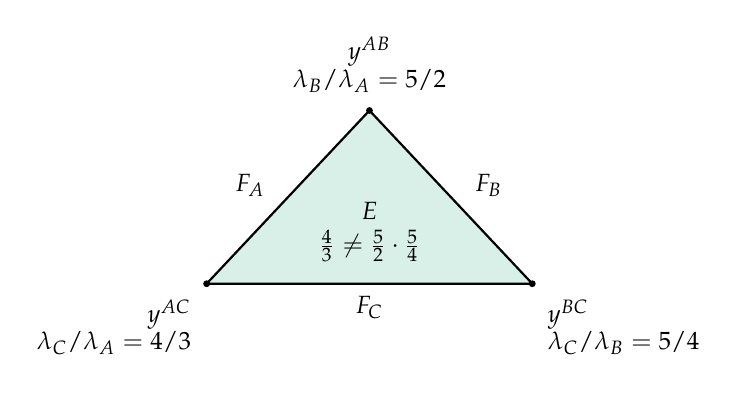
\begin{tikzpicture}[scale=0.88, every node/.style={font=\small}]
  \coordinate (AB) at (0,2.5);
  \coordinate (AC) at (-2.35,0);
  \coordinate (BC) at (2.35,0);
  \fill[clearinggreen] (AB)--(AC)--(BC)--cycle;
  \draw[thick] (AB)--(AC)--(BC)--cycle;
  \fill (AB) circle (1.4pt) (AC) circle (1.4pt) (BC) circle (1.4pt);
  \node at (0,1.05) {$E$};
  \node at (-1.72,1.42) {$F_A$};
  \node at (1.72,1.42) {$F_B$};
  \node at (0,-0.35) {$F_C$};
  \node[align=center,above=3pt] at (AB) {$y^{AB}$\\[-1pt]$\lambda_B/\lambda_A=5/2$};
  \node[align=right,below left=3pt] at (AC) {$y^{AC}$\\[-1pt]$\lambda_C/\lambda_A=4/3$};
  \node[align=left,below right=3pt] at (BC) {$y^{BC}$\\[-1pt]$\lambda_C/\lambda_B=5/4$};
  \node[font=\bfseries\small] at (0,0.55) {$\tfrac{4}{3}\ne\tfrac{5}{2}\cdot\tfrac{5}{4}$};
\end{tikzpicture}
\caption{Schematic scale transport in the three-facet log-affine market. Direct transport gives $\lambda_C/\lambda_A=4/3$, while transport through $B$ gives $(5/2)(5/4)=25/8$; no single diagonal scaling is compatible with all three ridges.}
\label{fig:three-facet-schematic}
\end{figure}

The last two relations imply $\lambda_C=25\lambda_A/8$, contradicting the first relation $\lambda_C=4\lambda_A/3$.

Equating the direct value of $\lambda_C/\lambda_A$ in \eqref{eq:symbolic-ridge-ratios} with the product of the other two ratios shows that, for this three-facet incidence pattern, consistency would require
\begin{equation}\label{eq:cycle-compatibility}
K_{12}K_{23}K_{31}=K_{13}K_{21}K_{32}.
\end{equation}
For \eqref{eq:K-matrix}, the two sides are $K_{12}K_{23}K_{31}=32$ and $K_{13}K_{21}K_{32}=75$.
\end{proof}

The obstruction is local: it uses the potential identity only on a strictly positive neighborhood of the displayed facet--ridge configuration, and it requires neither polyhedrality nor differentiability of $L$, nor continuity of $d$. Positivity of the ridge coordinates and scale coefficients, independence of the active normals, strictness of the inactive comparisons, and $32\ne75$ are open conditions, so the same incidence pattern and the same contradiction survive sufficiently small perturbations of the entries of $K$ within the log-affine class. Equation \eqref{eq:cycle-compatibility} is specific to this three-facet incidence pattern.

For comparison, some two-good log-affine markets are integrable. If two switching thresholds satisfy $\kappa_1<\kappa_2$, then in $y=1+p$ coordinates
\[
L(y)=\max\{0,\ \kappa_1y_2-y_1,\ y_1-\kappa_2y_2\}
\]
has gradients that are positive diagonal scalings of the excess-supply vectors $(-1,1)$, $(0,0)$, and $(1,-1)$. Thus some two-good log-affine markets are integrable, whereas the cycle obstruction used in \Cref{thm:potential} requires a third good.

\subsection{Proof of the universal potential boundary}\label{subsec:potential-proof}

\begin{proof}[Proof of \Cref{thm:potential}]
The implication (iii)$\Rightarrow$(i) is immediate. Under (i), every two-by-two unit-demand market with one unit of each good has a convex strictly positive equilibrium-price set by \eqref{eq:argmin-equilibrium}. \Cref{thm:geometry} leaves only the affine and common log-affine families. \Cref{lem:log-normalization} and \Cref{prop:holonomy} rule out the log-affine family. Hence (ii) holds.

For (ii)$\Rightarrow$(iii), use the scaled Lyapunov construction in \citet[Theorem~6.4]{okisato2026}:
\begin{equation}\label{eq:affine-L}
L(p)=
\sum_i\max_{x\in\Xcal_i}
\left\{\frac{v_i(x)}{\alpha_i}-\sum_j\beta_jp_jx_j\right\}
+\sum_j\beta_js_jp_j.
\end{equation}
The function is finite, polyhedral, and convex on $\R^M$ and hence on $\R_+^M$. At every interior price, Danskin's theorem gives
\[
\partial_+ L(p)=\diag(\beta)
\left(s-\sum_i\co D_i(p)\right).
\]
Thus \eqref{eq:potential-definition} holds with $d_j=1/\beta_j$.
\end{proof}

\subsection{Proof of Theorem~\ref{thm:lower-path}}\label{subsec:lower-path-proof}

Consider the market of \Cref{ex:two-good}. The ascending auction described in \Cref{subsec:path-relaxations} lets buyers choose subsets of goods, so extend each valuation to $\{0,1\}^2$ by $v_i(x)=\max\{v_{ij}:x_j=1\}$ and $v_i(0)=0$; this is the standard unit-demand valuation on $\{0,1\}^2$ and belongs to the substitutes class. At every interior price used below no buyer demands both goods, so the demand geometry is that of the unit-demand market. \ref{app:two-good-checks} records the remaining compatibility condition and exact demand and over-demand checks.

\begin{lemma}[Minimum equilibrium]\label{lem:path-minimum-equilibrium}
The minimum equilibrium price of \eqref{eq:path-market} is $\bar p=(5,5)$.
\end{lemma}

\begin{proof}
At $(5,5)$, buyer 1 is indifferent between the two singleton goods, buyer 2 strictly chooses good 1, and buyer 3 is indifferent between good 2 and the outside option. The allocation $x_1=e_2$, $x_2=e_1$, and $x_3=0$ therefore clears the market.

At any equilibrium, at least one of the three buyers receives the zero bundle. If this is buyer 1, outside-option optimality requires $p_1,p_2\ge10$. If it is buyer 2, it requires $p_1\ge10$ and $p_2\ge11/2$. If it is buyer 3, it requires $p_2\ge5$. Thus every equilibrium has $p_2\ge5$. If $p_1<5$ as well, buyers 1 and 2 both uniquely demand good 1: buyer 1 obtains more than $5$ from good 1 and at most $5$ from good 2, while buyer 2 obtains more than $5$ from good 1 and at most $1$ from good 2. One unit of good 1 cannot satisfy both unique demands. Hence every equilibrium also has $p_1\ge5$, proving the claim.
\end{proof}

The lower-box contradiction occurs at the interior price
\[
p^\circ=(1,1)<\bar p.
\]
Buyer 1 switches on $H_1=\{p:p_1-p_2=0\}$, whose normal is $n_1=(1,-1)$, and buyer 2 switches on $H_2=\{p:p_1-2p_2=-1\}$, whose normal is $n_2=(1,-2)$. Buyer 3 uniquely demands good 2 in a neighborhood of $p^\circ$. The two switching lines meet transversally. The three local cells used below are witnessed, for example, by
\[
p^{00}=(9/10,1),\qquad
p^{10}=(23/20,11/10),\qquad
p^{01}=(17/20,9/10),
\]
where buyers $(1,2)$ choose respectively $(1,1)$, $(2,1)$, and $(1,2)$. All three prices lie in the interior of the lower box.

\begin{lemma}[Polyhedral cell matching]\label{lem:polyhedral-cell-matching}
Let $L$ be finite and polyhedral convex on a full-dimensional convex domain, and let $C$ be a connected open set in the interior of the domain. If $\partial L(p)$ is a singleton for every $p\in C$, then $L$ is affine on $C$ and its gradient is constant there. If two such cells meet along a relatively open facet contained in a hyperplane with normal $n$, the difference of their gradients is parallel to $n$.
\end{lemma}

\begin{proof}
A polyhedral convex function is locally the maximum of finitely many affine functions on the interior of its domain. If two active affine functions at a point have different gradients, the subdifferential contains their nondegenerate convex hull. Hence, under the singleton hypothesis, all affine pieces active near a point have the same gradient and coincide there; the gradient is therefore locally constant on $C$. Since $C$ is connected, it is constant throughout $C$, and $L$ is affine there. Continuity makes the affine formulas of two adjacent cells agree on their common relatively open facet. Their difference is an affine function vanishing on that facet, so the difference of their gradients is normal to the containing hyperplane.
\end{proof}

\begin{lemma}[Interior subgradient compactness]\label{lem:subgradient-compactness}
Let $\Omega\subseteq\R^m$ be full-dimensional and convex, and let $L:\Omega\to\R$ be finite and convex. On every compact subset of $\operatorname{int}\Omega$, the subdifferentials of $L$ are uniformly bounded. Moreover, the graph of $\partial L$ is closed on $\operatorname{int}\Omega$.
\end{lemma}

\begin{proof}
Fix a compact $K\subset\operatorname{int}\Omega$. Choose $r>0$ such that $K+[-r,r]^m\subset\operatorname{int}\Omega$. Continuity of a finite convex function on the interior makes $L$ bounded in absolute value by some $M$ on this enlarged compact set. For $x\in K$, $g\in\partial L(x)$, and each coordinate $j$, the subgradient inequalities at $x\pm re_j$ give $|g_j|\le 2M/r$. This proves uniform boundedness. For closedness, if $x^n\to x\in\operatorname{int}\Omega$, $g^n\to g$, and $g^n\in\partial L(x^n)$, then for every $w\in\Omega$,
\[
L(w)\ge L(x^n)+g^n\cdot(w-x^n).
\]
Continuity at $x$ permits passage to the limit, yielding the subgradient inequality for $g$ at $x$.
\end{proof}

\begin{proof}[Proof of \Cref{thm:lower-path}(i)]
Fix a neighborhood $U$ of $p^\circ$ and suppose that a polyhedral convex $L:\R_+^2\to\R$ and a map $d:U\to\R_{++}^2$ satisfy \eqref{eq:potential-definition} at every $p\in U$. Since the identity restricts to every smaller neighborhood, we may take $U$ to be an open ball centered at $p^\circ$ that meets no switching line other than $H_1$ and $H_2$, so that these two lines cut $U$ into four open sectors and the intersection of $U$ with each demand cell is one sector, connected and open. In the cell where buyers 1 and 2 both choose good 1, excess supply is $(-1,0)$; in either adjacent cell where exactly one of them switches to good 2, excess supply is $(0,-1)$. By \Cref{lem:polyhedral-cell-matching}, the three constant cell gradients can be written
\[
g^{00}=(-a,0),\qquad
g^{10}=(0,-b),\qquad
g^{01}=(0,-c)
\]
for $a,b,c>0$. Across $H_1$, the jump $g^{10}-g^{00}=(a,-b)$ must be parallel to $(1,-1)$, so $b=a$. Across $H_2$, the jump $g^{01}-g^{00}=(a,-c)$ must be parallel to $(1,-2)$, so $c=2a$.

Taking sequences from the three cells to $p^\circ$ and applying the closed-graph part of \Cref{lem:subgradient-compactness} shows that
\[
(-a,0),\qquad(0,-a),\qquad(0,-2a)
\]
all belong to $\partial_+L(p^\circ)$. These three points are affinely independent, since the determinant of the two difference vectors is $-a^2\ne0$. Thus $\partial_+L(p^\circ)$ has affine dimension at least two.

At $p^\circ$, buyers 1 and 2 each demand $\{e_1,e_2\}$ and buyer 3 demands $e_2$. Hence
\begin{equation}\label{eq:path-Z-turn}
Z(p^\circ)
=(1,1)-e_2-\co\{e_1,e_2\}-\co\{e_1,e_2\}
=\co\{(-1,0),(1,-2)\}.
\end{equation}
This is a line segment. Every positive diagonal map is invertible and preserves affine dimension, so $\diag(d(p^\circ))^{-1}Z(p^\circ)$ remains one-dimensional. This contradicts the required equality with $\partial_+L(p^\circ)$. Since $p^\circ<\bar p$, some neighborhood $U$ of $p^\circ$ lies in the open box $(0,\bar p)$, and a lower-box diagonal potential restricted to such a $U$ would provide a pair of the kind just excluded; this proves the second sentence of (i).
\end{proof}

We next compute the auction path using only the Local Stability Condition.

\begin{lemma}[Forced locally stable path]\label{lem:forced-path}
Every execution from zero using directions that satisfy LSC follows \eqref{eq:realized-auction-path}, up to positive reparameterization of each segment. In particular, the outgoing direction ratio is forced to reset from $2{:}1$ to $1{:}1$ at $p^\circ=(1,1)$.
\end{lemma}

\begin{proof}
At $p=(0,0)$, the minimal demand sets are $\{e_1,e_2\}$ for buyer 1 and $\{e_2\}$ for buyers 2 and 3. The sets $\{2\}$ and $\{1,2\}$ both have over-demand value one, so the unique inclusion-minimal maximizer is $X^*=\{2\}$. The update therefore raises only $p_2$. For $p=(0,t)$ with $0<t<1/2$, the minimal demand profile is $(e_1,e_2,e_2)$ and $X^*=\{2\}$ remains unchanged. The first event occurs at
\[
p^a=(0,1/2),
\]
where buyer 2 becomes indifferent and the unique minimal maximizer becomes $X^*=\{1,2\}$.

Let $a=(a_1,a_2)\gg0$ be a candidate direction at $p^a$. Buyers 1 and 3 continue to demand goods 1 and 2, respectively, after every sufficiently small move. Buyer 2, who is indifferent at $p^a$, chooses good 1 if $a_1<2a_2$, chooses good 2 if $a_1>2a_2$, and remains indifferent if $a_1=2a_2$. In the first case both $\{1\}$ and the full set have over-demand value one, so the unique inclusion-minimal maximizer becomes $\{1\}$. In the second case the analogous conclusion holds with $\{2\}$. Under equality neither singleton is over-demanded while the full set has over-demand value one. Hence $X^*=\{1,2\}$ remains the unique minimal maximizer exactly when
\[
a_1=2a_2.
\]
The path therefore leaves $p^a$ on the ray $(2,1)$. Along this ray buyer 2 remains indifferent, while buyers 1 and 3 uniquely demand goods 1 and 2. The full set remains the unique minimal maximizer until the ray meets buyer 1's switching line $p_1=p_2$, which occurs at $p^\circ=(1,1)$.

Now let $a=(a_1,a_2)\gg0$ be a candidate direction at $p^\circ$. If $a_1<a_2$, buyer 1 selects good 1; buyer 2 also selects good 1 because $a_1<2a_2$, so the unique inclusion-minimal maximizer becomes $\{1\}$. If $a_1>a_2$, buyer 1 selects good 2; together with buyer 3, this makes the unique inclusion-minimal maximizer $\{2\}$, independently of buyer 2's choice. Only $a_1=a_2$ leaves buyer 1 indifferent while buyer 2 selects good 1 and buyer 3 selects good 2; then neither singleton is over-demanded and the full set remains the unique minimal maximizer. Thus LSC forces the outgoing ray $(1,1)$.

Along the diagonal from $(1,1)$ to $(5,5)$, buyer 1 remains indifferent, buyer 2 uniquely demands good 1, and buyer 3 uniquely demands good 2. The same argument forces the diagonal ray and keeps $X^*=\{1,2\}$ until $(5,5)$. There buyer 3's minimal demand becomes the zero bundle, no set is over-demanded, and the minimal maximizer is empty. This proves \eqref{eq:realized-auction-path}.
\end{proof}

\begin{proof}[Proof of \Cref{thm:lower-path}(ii)]
\Cref{lem:forced-path} proves the first sentence of (ii). For the second, suppose $L:\R_+^2\to\R$ is finite and convex and $d$ is proportional to $a^+$ on the final part of the incoming $(2,1)$ segment and at $p^\circ$, with \eqref{eq:potential-definition} holding there. Take a sequence $p^n$ on the open $(2,1)$ segment in \eqref{eq:realized-auction-path} converging to $p^\circ$. There buyer 1 uniquely demands good 1, buyer 2 ties, and buyer 3 uniquely demands good 2, so
\[
Z(p^n)=\co\{(-1,0),(0,-1)\}.
\]
Since $a^+(p^n)=(2,1)$, write $d(p^n)=c_n(2,1)$ with $c_n>0$. Then
\begin{equation}\label{eq:path-incoming-subdiff}
\partial_+L(p^n)
=\co\{(-\lambda_n/2,0),(0,-\lambda_n)\},
\qquad \lambda_n=1/c_n.
\end{equation}

At $p^\circ$, the outgoing direction is proportional to $(1,1)$, so $d(p^\circ)=c_\circ(1,1)$ for some $c_\circ>0$. By \eqref{eq:path-Z-turn},
\begin{equation}\label{eq:path-turn-subdiff}
\partial_+L(p^\circ)
=\co\{(-1/c_\circ,0),(1/c_\circ,-2/c_\circ)\}.
\end{equation}
Every vector in this segment lies on the affine line
\[
x_1+x_2=-1/c_\circ,
\]
which does not contain the origin.

By \Cref{lem:subgradient-compactness}, the incoming subgradients are locally bounded and their graph is closed. Thus $(\lambda_n)$ has a convergent subsequence, say $\lambda_n\to\lambda\ge0$. If $\lambda=0$, either endpoint in \eqref{eq:path-incoming-subdiff} converges to zero, and closedness gives $0\in\partial_+L(p^\circ)$, contradicting \eqref{eq:path-turn-subdiff}. If $\lambda>0$, closedness places both $(-\lambda/2,0)$ and $(0,-\lambda)$ in $\partial_+L(p^\circ)$. Their coordinate sums are $-\lambda/2$ and $-\lambda$, so they cannot both lie on the same affine line $x_1+x_2=-1/c_\circ$. This is again a contradiction. A posted-price potential along $\Gamma$ would provide such a pair $(L,d)$.
\end{proof}

Write $q_{ij}(p_j)=\beta_{ij}p_j$ for the linear schedules in \eqref{eq:path-market}, so that $\beta_{22}=2$ and every other slope equals one. Both conclusions of \Cref{thm:lower-path} persist under every sufficiently small admissible perturbation of the six singleton values and the six slopes that keeps the schedules linear. Admissibility includes $v_{31}\ge0$, which keeps buyer 3's extension to $\{0,1\}^2$ monotone and the ascending auction defined, so the neighborhood is one-sided in that coordinate. \Cref{lem:two-good-robustness} in \ref{app:two-good-checks} states sufficient conditions on the perturbed primitives and proves the claim, including that the terminal price remains the minimum equilibrium. The dimension contradiction is preserved by the distinct switching normals, and the closed-graph contradiction by the incompatible incoming and outgoing rays.

\subsection{Proof of the piecewise-linear boundary}\label{subsec:piecewise}

The proof of \Cref{cor:piecewise} has two steps: vanishing local slope minors force a common effective-price coordinate, and any kink in that coordinate bends an indifference locus, yielding two equilibrium prices with a nonequilibrium midpoint. The common coordinate must therefore be affine; the smooth logarithmic coordinate escapes because its difference level sets remain straight. \ref{app:piecewise-factorization} completes the factorization and kink details.

\section{The effective-price objective}\label{sec:effective}

\begin{proof}[Proof of \Cref{prop:effective}]
After division by $\alpha_i$, buyer $i$ maximizes $v_i(x)/\alpha_i-r\cdot x$. The pointwise-maximum representation and Danskin's theorem give convexity and the subdifferential formula \eqref{eq:Lhat-subdiff}, while finiteness and polyhedrality follow from the finiteness of each $\Xcal_i$. For $r\in\mathcal R_Q$, the condition $0\in\partial\widehat L(r)$ is equivalent to convexified clearing at $Q^{-1}(r)$. Positive rescaling preserves $M^\natural$-concavity, so \Cref{lem:convexified-clearing} converts this condition to exact clearing and gives \eqref{eq:effective-minimizers}.
\end{proof}

To compare this objective with posted-price convexity, define the pullback $\Phi(p)=\widehat L(Q(p))$.

For any $p^0,p^1\in\R_+^M$, the function $t\mapsto\Phi(p(t))$ is convex on $[0,1]$ along the effective-price segment
\begin{equation}\label{eq:geodesic}
p(t)=Q^{-1}\big((1-t)Q(p^0)+tQ(p^1)\big),
\qquad t\in[0,1],
\end{equation}
because $Q(p(t))$ is affine in $t$ and $\widehat L$ is convex. Along such a segment, the one-sided derivatives of $\Phi$ are monotone, so an interval whose one-sided derivative signs bracket zero can be bisected to a segment minimizer. Clearing follows only if the segment contains a global minimizer of $\widehat L$, so the bisection is a segment method.

If each $Q_j$ is $C^1$ with positive derivative, write $J_Q(p)=\diag(Q'_j(p_j))_{j\in M}$. At every $p\in\R_{++}^M$ where $\widehat L$ is differentiable at $Q(p)$, let $z(p)=\nabla\widehat L(Q(p))$ denote the unique excess-supply vector. The chain rule and the pullback of effective-price descent $\dot r=-z$ give
\begin{equation}\label{eq:smooth-pullback}
\nabla_p\Phi(p)=J_Q(p)^\top z(p),
\qquad
\dot p=-J_Q(p)^{-1}z(p).
\end{equation}
Thus overdemanded goods rise at a speed inversely proportional to their marginal effective-payment slope. This is ordinary gradient descent after the coordinate change $r=Q(p)$, written back in posted prices.

Under substitutes valuations, unbounded ranges, equilibrium existence, and square-summable diminishing steps, projected subgradient adjustment on $\widehat L$ converges to a minimizer, so $p^t=Q^{-1}(r^t)$ converges to an equilibrium price; \ref{app:adjustment} states and proves this standard result as \Cref{lem:adjustment-convergence}. Convergence is asymptotic and selects no particular equilibrium.

The three-good log-affine market of \Cref{prop:holonomy} shows the distinction. Its effective-price objective is convex and its minimizers pull back to a convex posted-price equilibrium set, yet the market admits no posted-price diagonal potential. Convexity of the minimizer set alone does not imply cyclic monotonicity of the scaled excess-supply correspondence.

\section{Discussion and conclusion}\label{sec:discussion}

For smooth payments, affine rank-one schedules preserve both universal posted-price properties, while the common log-affine family preserves equilibrium convexity but not global posted-price integrability. No other smooth family preserves the second property. The separation is off equilibrium: exponentiation preserves the affine description of substitutes equilibrium-price sets, whereas the three-facet obstruction prevents local adjustment scales from closing around a cycle. For continuous finitely piecewise-linear schedules, affine rank one characterizes both universal properties, so a genuine kink removes the universal guarantee of one posted-price potential.

The two-good market of \Cref{ex:two-good} gives this global requirement local content. The diagonal identity fails for every polyhedral potential in every neighborhood of an interior price below the minimum equilibrium price, and along the realized locally stable path the forced reset separates the incoming scale from the outgoing scale, so that no finite convex function in posted prices serves both regimes. The general auction of \citet{okisato2026} needs no such potential, because it recomputes its direction whenever the over-demanded set changes.

\Cref{prop:effective} gives general separable schedules the convex objective $\widehat L$ in effective prices. This coordinate result complements the posted-price classification, since common log-affine schedules retain $\widehat L(r)$ while failing the posted-price potential test. Likewise, a bracket schedule may support cell-specific potentials that are replaced at slope changes while lying outside the universal global class.

Affine rank-one payments admit one global convex objective directly in posted prices. Common log-affine payments preserve equilibrium averaging but require effective prices for the general convex objective. More general separable payments retain only the effective-price result, while general nonseparable piecewise-linear frictions retain finite ascending computation. Extending the local scale-compatibility analysis to arbitrary clearing-cell complexes remains open.
\clearpage
\appendix
\renewcommand{\thelemma}{\Alph{section}.\arabic{lemma}}
\setcounter{table}{0}
\setcounter{figure}{0}

\section{Local slope obstruction and marginal factorization}\label{app:factorization}

\begin{proof}[Proof of \Cref{prop:local-minor}]
Set $\delta_h=q_{hj}(t)-q_{h\ell}(u)$ for $h\in\{i,k\}$ and define
\begin{equation}\label{eq:H-smooth}
H(x,y)=
\begin{pmatrix}
q_{ij}(x)-q_{i\ell}(y)-\delta_i\\
q_{kj}(x)-q_{k\ell}(y)-\delta_k
\end{pmatrix},
\qquad
DH(t,u)=
\begin{pmatrix}
q'_{ij}(t)&-q'_{i\ell}(u)\\
q'_{kj}(t)&-q'_{k\ell}(u)
\end{pmatrix}.
\end{equation}
The hypothesis makes this Jacobian nonsingular. For small $\eps>0$, the inverse function theorem gives prices $p^A,p^B$ near $(t,u)$. Writing $J=DH(t,u)$, the relevant expansions are
\begin{align*}
H(p^A)&=(-3\eps,\eps),
&H(p^B)&=(\eps,-3\eps),\\
p^A-(t,u)&=J^{-1}(-3\eps,\eps)+o(\eps),
&p^B-(t,u)&=J^{-1}(\eps,-3\eps)+o(\eps),\\
H\left(\frac{p^A+p^B}{2}\right)&=(-\eps,-\eps)+o(\eps),
\end{align*}
which is strictly negative componentwise for sufficiently small $\eps$.

Give buyer $h\in\{i,k\}$ singleton-value difference $v_{hj}-v_{h\ell}=\delta_h$ and add a common large constant to both singleton values so that the outside option is strictly dominated nearby. Buyer $h$ chooses $j$ when $H_h<0$ and $\ell$ when $H_h>0$. At $p^A$ the two buyers split the goods; at $p^B$ they split them in the opposite way. Both prices clear one unit of each good. At their midpoint both buyers choose $j$, so the midpoint does not clear.
\end{proof}

\begin{proof}[Proof of \Cref{lem:smooth-factorization}]
Fix a reference buyer $i_0$, a reference good $j_0$, and a reference price $t_0>0$. Set
\[
\alpha_i=\frac{q'_{ij_0}(t_0)}{q'_{i_0j_0}(t_0)}>0.
\]
For any good $j\ne j_0$ and price $t>0$, apply \eqref{eq:all-minors-zero} to buyers $i,i_0$, goods $j,j_0$, and prices $t,t_0$:
\[
q'_{ij}(t)q'_{i_0j_0}(t_0)
=q'_{ij_0}(t_0)q'_{i_0j}(t).
\]
Hence $q'_{ij}(t)=\alpha_iq'_{i_0j}(t)$. For $j=j_0$, use any other good $\ell$ and apply the same identity first at $(t,u)$ and then at $(t_0,u)$ to see that the ratio $q'_{ij_0}(t)/q'_{i_0j_0}(t)$ equals $\alpha_i$ for every $t$. Define $Q_j'=q'_{i_0j}$ and $Q_j(0)=0$. Since $q_{ij}(0)=0$, integration yields $q_{ij}=\alpha_iQ_j$.
\end{proof}

\section{Straight indifference sets and affine semigroups}\label{app:straight-level}

Fix goods $j,k$, prices $x_0,y_0>0$, and $c=Q_j(x_0)-Q_k(y_0)$. By the implicit function theorem, the level set \eqref{eq:level-set} is locally the graph $y=T(x)$ because $Q_k'>0$. Give two unit-demand buyers effective singleton values $w_j,w_k$ with $w_j-w_k=c$, and add the same large constant to both values. In a small rectangle around $(x_0,y_0)$, both buyers strictly prefer some good to the outside option. On the graph they are both indifferent, so one can assign one buyer to each good and clear. On either side they strictly agree on one good, so the market does not clear. Thus the local equilibrium set is precisely the graph.

If this graph is a convex subset of $\R^2$, the chord between any two nearby graph points lies in the graph. Writing $T((1-t)x_1+tx_2)=(1-t)T(x_1)+tT(x_2)$ for all nearby $x_1,x_2$ and $t\in[0,1]$ shows that $T$ is locally affine. Continuity and overlap of the local intervals make the affine coefficients agree on each connected component of the domain. Since the domain of $T_{jk,c}$ is an interval, the map is affine throughout that domain.

Fix $x_0$ in the domain of $S_{j,t}$ and another good $k$. Choose $\rho$ in the interior of the range of $Q_k$, and set $c_1=Q_j(x_0)-\rho$ and $c_2=-t-c_1$. Then, near $x_0$,
\begin{equation}\label{eq:translation-composition}
S_{j,t}=T_{kj,c_2}\circ T_{jk,c_1}.
\end{equation}
Both cross-good maps are locally affine. Overlapping neighborhoods make the coefficients agree, so $S_{j,t}$ is affine on its full interval domain. Its coefficients are continuous in $t$, and effective-price addition gives \eqref{eq:semigroup-identities} whenever $t,u,t+u<R_j$.

The continuous multiplicative equation for $a_j$ gives $a_j(t)=e^{\gamma_jt}$ for some $\gamma_j\in\R$, even if the parameter interval is finite. If $\gamma_j=0$, the equation for $b_j$ is the continuous additive Cauchy equation, so $b_j(t)=c_jt$ for some $c_j>0$. If $\gamma_j\ne0$, commutativity gives
\[
\bigl(e^{\gamma_jt}-1\bigr)b_j(u)
=\bigl(e^{\gamma_ju}-1\bigr)b_j(t),
\]
and hence $b_j(t)=c_j(e^{\gamma_jt}-1)$. If $R_j<\infty$, strict monotonicity requires $Q_j^{-1}(t)=b_j(t)\to\infty$ as $t\uparrow R_j$, whereas either candidate remains finite. Thus $R_j=\infty$. Since $b_j$ is then positive and unbounded, the nonzero-rate case has $\gamma_j>0$ and $c_j>0$. Inverting $b_j$ gives \eqref{eq:inverse-two-forms}.

For cross-good compatibility, $T_{jk,0}=Q_k^{-1}\circ Q_j$ is affine and fixes zero, hence is linear. A linear coordinate and a logarithmic coordinate cannot be related by such a map. If both are logarithmic, direct substitution gives
\[
Q_k^{-1}(Q_j(x))
=c_k\left[\left(1+\frac{x}{c_j}\right)^{\gamma_k/\gamma_j}-1\right],
\]
which is affine only when $\gamma_k=\gamma_j$. Thus all goods use the same branch and the logarithmic branch has one common rate.

\section{Convexified clearing and Walrasian price polyhedra}\label{app:walrasian}

\begin{lemma}[Convexified clearing under substitutes]\label{lem:convexified-clearing}
Suppose each $\widetilde v_i$ is $M^\natural$-concave. For every collection $a=(a_i)_{i\in N}$ and every integer supply vector $s\in\Z^M$,
\[
s\in\sum_{i\in N}D_i[a_i]
\quad\Longleftrightarrow\quad
s\in\sum_{i\in N}\co D_i[a_i].
\]
\end{lemma}

The lemma follows from $M^\natural/L^\natural$ conjugacy \citep[Theorem~4.5]{murota2016} and integer decomposition for Minkowski sums of the associated integral generalized polymatroids \citep[equation~(3.1), Theorem~3.1, and Example~3.1]{murotatamura2024}. It makes $0\in Z(p)$ equivalent to exact clearing. The next lemma supplies the second discrete-convex input: nonempty full-space equilibrium sets have coordinate-and-difference-bound representations.

\begin{lemma}[Full-space Walrasian price polyhedron]\label{lem:walrasian-price-polyhedron}
Suppose each $\widetilde v_i$ is $M^\natural$-concave and let $\alpha_i>0$. Define
\[
\mathcal L(r)=
\sum_i\max_{x\in\Xcal_i}
\left\{\frac{v_i(x)}{\alpha_i}-r\cdot x\right\}
+s\cdot r,
\qquad r\in\R^M;
\]
this function coincides with the effective-price objective \eqref{eq:Lhat}, and the separate symbol emphasizes that the lemma requires no payment structure. Then $\mathcal L$ is a finite polyhedral continuous $L^\natural$-convex function and
\[
\partial\mathcal L(r)
=s-\sum_i\co\argmax_{x\in\Xcal_i}
\left\{\frac{v_i(x)}{\alpha_i}-r\cdot x\right\}.
\]
If its full-space minimizer set is nonempty, that set is the full-space exact-clearing price set and is a continuous $L^\natural$-convex polyhedron. Consequently, there are possibly infinite bounds $\underline r_j,\overline r_j,c_{jk}$ such that
\[
\argmin_{r\in\R^M}\mathcal L(r)=
\left\{r\in\R^M:
\underline r_j\le r_j\le\overline r_j,
\quad r_j-r_k\le c_{jk}\ \text{for all }j,k
\right\}.
\]
Constraints with an infinite bound are vacuous and are omitted.
\end{lemma}

\begin{proof}
Conjugacy and closure under sums and linear terms give $L^\natural$-convexity, while Danskin's theorem gives the subdifferential formula \citep[Theorems~7.10 and 8.2]{murota2016}. The minimizer condition is convexified clearing; \Cref{lem:convexified-clearing} converts it to exact clearing. The minimizer set inherits continuous $L^\natural$-convexity, and its coordinate-and-difference-bound representation follows from \citet[Theorem~2.2(2)]{moriguchimurota2023}.
\end{proof}

\section{The three-good log-affine market}\label{app:facets}

\begin{lemma}[Log-affine normalization]\label{lem:log-normalization}
Let $B=\diag(\beta_1,\ldots,\beta_m)$ and suppose payments have the form \eqref{eq:log-family}. Given normalized unit-demand values $\bar v_{ij}$, set $v_{ij}=\alpha_i\bar v_{ij}$, $\bar p=Bp$, and $y=\one+\bar p$. Demand in the original market at $p$ equals demand in the normalized log-affine market with values $\bar v_{ij}$ and payments $\log y_j$. The original market admits a finite convex, respectively polyhedral, diagonal potential on $\R_+^M$ if and only if the normalized market in $\bar p$-coordinates does.
\end{lemma}

\begin{proof}
Dividing buyer $i$'s utility by $\alpha_i$ gives the demand claim. For a potential pair $(L,d)$ satisfying \Cref{def:potential} in $p$-coordinates, define $\overline L:\R_+^M\to\R$ by
\[
\overline L(\bar p)=L(B^{-1}\bar p).
\]
For $\bar p\in\R_{++}^M$, let $\overline Z(\bar p)=Z(B^{-1}\bar p)$ and $\overline d_j(\bar p)=\beta_jd_j(B^{-1}\bar p)$. The affine chain rule gives
\[
\partial_+\overline L(\bar p)
=B^{-1}\partial_+ L(B^{-1}\bar p)
=\diag(\overline d(\bar p))^{-1}\overline Z(\bar p).
\]
The change of coordinates preserves finite-valued convexity and polyhedrality. Applying the inverse affine map proves the converse.
\end{proof}

For buyer $i$ switching from good $j$ to good $k$, define
\begin{equation}\label{eq:facet-normal-general}
n_{i,jk}=\frac{e_j}{K_{ij}}-\frac{e_k}{K_{ik}}.
\end{equation}
The buyer chooses $j$ on $n_{i,jk}\cdot y<0$ and $k$ on $n_{i,jk}\cdot y>0$. At a point $y$, buyer $i$'s three normalized costs are $(y_1/K_{i1},y_2/K_{i2},y_3/K_{i3})$. Direct substitution at the three ridges gives
\begin{center}
\scriptsize
\begin{tabular}{@{}ccccc@{}}
\toprule
Ridge & $y$ & Buyer 1 costs & Buyer 2 costs & Buyer 3 costs\\
\midrule
$AC$ & $(15,8,12)$ & $(15,4,4)$ & $(3,4,3)$ & $(15/4,8/5,12)$\\
$AB$ & $(16,20,30)$ & $(16,10,10)$ & $(16/5,10,15/2)$ & $(4,4,30)$\\
$BC$ & $(20,25,16)$ & $(20,25/2,16/3)$ & $(4,25/2,4)$ & $(5,5,16)$\\
\bottomrule
\end{tabular}
\end{center}
Thus exactly the two named switches are active at each ridge: buyers 1 and 2 at $AC$, buyers 1 and 3 at $AB$, and buyers 2 and 3 at $BC$. Every other comparison is strict.

The midpoints of the corresponding ridge pairs are
\[
x_A=\left(\frac{31}{2},14,21\right),\qquad
x_B=\left(18,\frac{45}{2},23\right),\qquad
x_C=\left(\frac{35}{2},\frac{33}{2},14\right).
\]
At $x_A$ only buyer 1 ties between goods 2 and 3; at $x_B$ only buyer 3 ties between goods 1 and 2; and at $x_C$ only buyer 2 ties between goods 1 and 3. All remaining comparisons are strict. Continuity therefore gives a relative-open two-dimensional neighborhood of each midpoint in its switching hyperplane with no other active comparison. More generally, every inactive-good cost gap is nonnegative at both endpoints of its ridge-to-ridge segment and never vanishes at both. Because each gap is affine in $y$, it is strictly positive at every interior point of the open segment.

Full-dimensional witnesses for the four unique-demand cells are
\begin{equation}\label{eq:cell-witnesses}
\begin{array}{c|cccc}
X&E&A&B&C\\ \hline
y&(51,53,58)&(31,27,42)&(35,45,46)&(36,33,28)\\
(x_1,x_2,x_3)&(3,1,2)&(2,1,2)&(3,1,1)&(3,3,2).
\end{array}
\end{equation}
All choices in \eqref{eq:cell-witnesses} are strict. The first point equals $y^{AC}+y^{AB}+y^{BC}$ and is the clearing-cell witness used above. Every displayed coordinate exceeds one, so $p=y-\one$ is strictly positive without further rescaling. Taking $C_0=\log 100$ makes the chosen singleton utility positive at every displayed point and on all three closed ridge-to-ridge segments: throughout this compact configuration the best normalized cost is strictly below $100$. The same remains true in sufficiently small neighborhoods. Hence the outside option is irrelevant everywhere used in the proof. The accompanying script \texttt{verify\_three\_facet\_\allowbreak certificate.py} performs all displayed comparisons, normal-orientation checks, zero-coordinate ray-isolation checks, and cycle arithmetic exactly over the rationals.

\section{Facet-to-ridge endpoint transport}\label{app:cell-gradient}

Under the hypotheses of \Cref{lem:ridge-transport}, let $(L_p,d_p)$ satisfy \Cref{def:potential} and write $Z_p$ for excess supply. Make the coordinate change used in \Cref{prop:holonomy}: define $L_y:[1,\infty)^3\to\R$ and, on $y\in(1,\infty)^3$, define $d_y$ and $Z_y$ by
\begin{align*}
L_y(y)&=L_p(y-\one),
&d_y(y)&=d_p(y-\one),
&Z_y(y)&=Z_p(y-\one).
\end{align*}
Translation preserves finiteness and convexity, and
\[
\partial_+ L_y(y)=\partial_+ L_p(y-\one)
=\diag(d_y(y))^{-1}Z_y(y).
\]
We suppress the subscripts below.

Let $E_+=E\cap(1,\infty)^3$. On this clearing chamber, $Z=\{0\}$. On each facet patch and at each ridge, the clearing allocation remains demanded, so $0\in Z$. Every point used below is therefore a global minimizer of $L$.

At each ridge the two named buyer switches are independent. Therefore the convexified excess-supply sets, and hence the ridge subdifferentials, are
\begin{align*}
\partial L(y^{AC})&=[0,u_A^{AC}]+[0,u_C^{AC}],\\
\partial L(y^{AB})&=[0,u_A^{AB}]+[0,u_B^{AB}],\\
\partial L(y^{BC})&=[0,u_B^{BC}]+[0,u_C^{BC}].
\end{align*}
Every vector in these subdifferentials is normal to the local closure of the clearing chamber $E_+$. Indeed, if $v\in\partial L(y^\rho)$ and $x\in E_+$, then both points minimize $L$, so the subgradient inequality gives $v\cdot(x-y^\rho)\le0$; passing to the closure yields $v\in N_{\overline E_+}(y^\rho)$.

Locally, the closure of the clearing cell is described by
\[
n_1\cdot y\ge0,\qquad n_2\cdot y\le0,\qquad n_3\cdot y\ge0.
\]
The inactive inequality is strict at each ridge. Consequently,
\begin{center}
\small
\begin{tabular}{@{}clll@{}}
\toprule
Ridge & Normal cone & Zero coordinates & Forced rays\\
\midrule
$AC$ & $\operatorname{cone}(-n_1,n_2)$
& $(u_A^{AC})_1=0$, $(u_C^{AC})_2=0$
& $u_A^{AC}\in\R_+(-n_1)$, $u_C^{AC}\in\R_+n_2$\\
$AB$ & $\operatorname{cone}(-n_1,-n_3)$
& $(u_A^{AB})_1=0$, $(u_B^{AB})_3=0$
& $u_A^{AB}\in\R_+(-n_1)$, $u_B^{AB}\in\R_+(-n_3)$\\
$BC$ & $\operatorname{cone}(-n_3,n_2)$
& $(u_B^{BC})_3=0$, $(u_C^{BC})_2=0$
& $u_B^{BC}\in\R_+(-n_3)$, $u_C^{BC}\in\R_+n_2$\\
\bottomrule
\end{tabular}
\end{center}
For example, at $AC$ the first coordinate of $n_2$ is nonzero whereas that of $-n_1$ is zero, so the zero first coordinate of $u_A^{AC}$ eliminates the $n_2$ coefficient. The second coordinate analogously isolates $u_C^{AC}$ on the $n_2$ ray. The other rows follow identically. In each row the two generating normals are linearly independent.

\begin{proof}[Proof of \Cref{lem:ridge-transport}]
We show the $A$--$AC$ incidence; the other five are identical. Take $x_A\in F_A$. Both $x_A$ and $y^{AC}$ minimize $L$, and $g_A\in\partial L(x_A)$ is normal to their common switching hyperplane. Hence, for every $w\in[1,\infty)^3$,
\[
L(w)\ge L(x_A)+g_A\cdot(w-x_A)
     =L(y^{AC})+g_A\cdot(w-y^{AC}),
\]
so $g_A\in\partial L(y^{AC})$.

The facet identity $\partial L(x_A)=\diag(d(x_A))^{-1}[0,z_A]$, together with facet rigidity, places $g_A$ on $\R_+(-n_1)$. The table places $u_A^{AC}$ on the same ray and $u_C^{AC}$ on the linearly independent ray $\R_+n_2$. Since
\[
\partial L(y^{AC})=[0,u_A^{AC}]+[0,u_C^{AC}],
\]
the unique two-ray decomposition of $g_A$ has zero $u_C^{AC}$ coefficient. Thus $g_A\in[0,u_A^{AC}]$. Conversely, $u_A^{AC}$ is a ridge subgradient normal to the $A/E$ switching hyperplane. The same supporting-hyperplane argument, now from $y^{AC}$ to $x_A$, gives
\[
u_A^{AC}\in\partial L(x_A)=[0,g_A].
\]
The two segment inclusions and $g_A\ne0$ imply $u_A^{AC}=g_A$. Repeating the argument at every facet--ridge incidence gives all six identities in the lemma.
\end{proof}

\section{Piecewise-linear factorization}\label{app:piecewise-factorization}

\begin{lemma}[Piecewise-linear factorization]\label{lem:piecewise-factorization}
Under the assumptions of \Cref{cor:piecewise}, suppose all local $2\times2$ slope minors vanish on every product of open linearity intervals. Then there are constants $\alpha_i>0$ and common continuous, strictly increasing, finitely piecewise-linear schedules $Q_j$ such that $q_{ij}=\alpha_iQ_j$.
\end{lemma}

\begin{proof}
Fix a reference buyer $i_0$, good $j_0$, and a regular reference price. The same ratio argument as in \ref{app:factorization} shows that at every regular price
\[
q'_{ij}(p)=\alpha_i\sigma_j(p)
\]
with constants $\alpha_i>0$. The slope identity holds at every common regular point and hence almost everywhere. Continuous finitely piecewise-linear functions are absolutely continuous, so integration from zero gives $q_{ij}=\alpha_iQ_j$ for common continuous piecewise-linear schedules $Q_j$.
\end{proof}

\begin{proof}[Proof of \Cref{cor:piecewise}]
Clearly (ii) implies (i). Suppose (i) holds. On every open linearity rectangle, the local-minor argument in \Cref{prop:local-minor} is exact rather than asymptotic, so all local slope minors vanish. \Cref{lem:piecewise-factorization} then yields $q_{ij}=\alpha_iQ_j$. If some $Q_j$ is non-affine, it has a kink at $x_0$. Choose another good $k$ and a regular $y_0$, and set $c=Q_j(x_0)-Q_k(y_0)$. The local graph $Q_j(x)-Q_k(y)=c$ inherits a kink because $Q_k^{-1}$ is locally affine around $y_0$. Its graph is not convex as a set, and the two-identical-buyers construction in \ref{app:straight-level} yields two strictly positive clearing prices with a nonclearing midpoint. Hence every $Q_j$ is affine, proving (iv).

If (iii) holds, \eqref{eq:argmin-equilibrium} makes the strictly positive equilibrium-price set convex on every restriction. The local-minor and kink constructions above use only strictly positive prices, so the same argument again gives (iv). Finally, (iv) implies (ii) by \Cref{thm:geometry} and implies (iii) by the potential in \eqref{eq:affine-L}. Thus all four statements are equivalent.
\end{proof}

\section{Diminishing-step effective-price adjustment}\label{app:adjustment}

\begin{lemma}[Diminishing-step effective-price adjustment]\label{lem:adjustment-convergence}
Suppose \eqref{eq:general-separable} holds, every $Q_j$ is unbounded, each $\widetilde v_i$ is $M^\natural$-concave, and equilibrium exists. Start from $r^0\in\R_+^M$. At each date $t$, choose $x_i^t\in D_i(Q^{-1}(r^t))$, set $z^t=s-\sum_i x_i^t$, and update
\begin{equation}\label{eq:projected-adjustment}
r^{t+1}=\Pi_{\R_+^M}\bigl(r^t-\eta_t z^t\bigr),
\end{equation}
where $\Pi_{\R_+^M}$ is Euclidean projection, $\eta_t>0$, $\sum_t\eta_t=\infty$, and $\sum_t\eta_t^2<\infty$. Then $r^t$ converges to a minimizer $r^*$ of $\widehat L$ in $\R_+^M$, and $p^t=Q^{-1}(r^t)$ converges to an equilibrium price $p^*=Q^{-1}(r^*)$.
\end{lemma}

The update raises the effective prices of overdemanded goods and lowers those of underdemanded goods, subject to projection. For the two families classified in \Cref{thm:geometry}, the unbounded-range hypothesis is automatic because the proof of that theorem derives $R_j=\infty$.

\begin{proof}
Unboundedness makes each $Q_j$ a homeomorphism from $\R_+$ onto $\R_+$, so $\mathcal R_Q=\R_+^M$. By \eqref{eq:Lhat-subdiff}, every realized excess-supply vector $z^t$ belongs to $\partial\widehat L(r^t)$. These subgradients are uniformly bounded because every $\Xcal_i$ is finite; fix $G$ with $\lVert z^t\rVert\le G$. Equilibrium existence and \Cref{prop:effective} make
\[
S=\argmin_{r\in\R^M}\widehat L(r)\cap\R_+^M
\]
nonempty. For any $r^*\in S$, projection nonexpansiveness and the subgradient inequality give
\begin{equation}\label{eq:adjustment-descent}
\lVert r^{t+1}-r^*\rVert^2
\le
\lVert r^t-r^*\rVert^2
-2\eta_t\bigl(\widehat L(r^t)-\widehat L(r^*)\bigr)
+\eta_t^2G^2.
\end{equation}
Because $\sum_t\eta_t^2<\infty$, the iterates are quasi-Fej\'er relative to $S$, and summing \eqref{eq:adjustment-descent} yields
$\sum_t\eta_t(\widehat L(r^t)-\min\widehat L)<\infty$.
Since $\sum_t\eta_t=\infty$, some subsequence has objective values converging to the minimum. Boundedness, continuity of $\widehat L$, and the quasi-Fej\'er inequality then imply that the whole sequence converges to a point of $S$. Continuity of $Q^{-1}$ and \eqref{eq:effective-minimizers} give the posted-price conclusion.
\end{proof}

\section{The two-good market: exact checks and robustness}\label{app:two-good-checks}

The valuations of \Cref{ex:two-good}, extended to $\{0,1\}^2$ as in \Cref{subsec:lower-path-proof}, are unit-demand valuations and hence belong to the substitutes class. Every payment is linear with a positive slope and vanishes at zero. The remaining condition of \citet{okisato2026}, that some price $\kappa\ge0$ satisfies $q_{ij}(\kappa)=v_i(e_j)$, holds with $\kappa=v_{ij}/q'_{ij}$, and for buyer 3 and good 1 with $\kappa=0$.

\Cref{tab:path-checks} records the minimal demand sets and over-demand values on the path.
\begin{table}[!ht]
\centering
\caption{Minimal demand sets and over-demand values along the realized auction path of the market in \eqref{eq:path-market}. Here $M=\{1,2\}$ and braces around two singleton bundles denote a tie.}
\label{tab:path-checks}
\small
\begin{tabular}{@{}llllrrrl@{}}
\toprule
Price region & $\check D_1$ & $\check D_2$ & $\check D_3$
& $O(\{1\})$ & $O(\{2\})$ & $O(M)$ & $X^*$\\
\midrule
$(0,0)$ & $\{e_1,e_2\}$ & $e_2$ & $e_2$ & $-1$ & $1$ & $1$ & $\{2\}$\\
$(0,t)$, $0<t<1/2$ & $e_1$ & $e_2$ & $e_2$ & $0$ & $1$ & $1$ & $\{2\}$\\
$(0,1/2)$ & $e_1$ & $\{e_1,e_2\}$ & $e_2$ & $0$ & $0$ & $1$ & $M$\\
$(2t,1/2+t)$, $0<t<1/2$ & $e_1$ & $\{e_1,e_2\}$ & $e_2$ & $0$ & $0$ & $1$ & $M$\\
$(1,1)$ & $\{e_1,e_2\}$ & $\{e_1,e_2\}$ & $e_2$ & $-1$ & $0$ & $1$ & $M$\\
$(1+t,1+t)$, $0<t<4$ & $\{e_1,e_2\}$ & $e_1$ & $e_2$ & $0$ & $0$ & $1$ & $M$\\
$(5,5)$ & $\{e_1,e_2\}$ & $e_1$ & $0$ & $0$ & $-1$ & $0$ & $\varnothing$\\
\bottomrule
\end{tabular}
\end{table}
The entries follow by direct utility comparison. At $p^a=(0,1/2)$ and at $p^\circ=(1,1)$, where the update direction changes, the strict and equality cases for a candidate direction give the three demand profiles enumerated in the proof of \Cref{lem:forced-path}.

\subsection*{Robustness of the two-good obstructions}

A perturbed market is a pair $\theta=(v,\beta)$ of a value matrix $v=(v_{ij})$ and a slope matrix $\beta=(\beta_{ij})$, with $i\in\{1,2,3\}$, $j\in\{1,2\}$, and payments $q_{ij}(p_j)=\beta_{ij}p_j$. Write $\theta^0$ for the market of \Cref{ex:two-good}. When $\beta_{12}\beta_{21}\ne\beta_{11}\beta_{22}$, set
\begin{equation}\label{eq:perturbed-anchors}
p^a(\theta)=\Bigl(0,\ \tfrac{v_{22}-v_{21}}{\beta_{22}}\Bigr),
\qquad
\bar p_2(\theta)=\frac{v_{32}}{\beta_{32}},
\qquad
\bar p_1(\theta)=\frac{v_{11}-v_{12}+\beta_{12}\,\bar p_2(\theta)}{\beta_{11}},
\end{equation}
and let $p^\circ(\theta)$ be the unique solution of the two switching equations
\begin{equation}\label{eq:perturbed-crossing}
\beta_{11}p_1-\beta_{12}p_2=v_{11}-v_{12},
\qquad
\beta_{21}p_1-\beta_{22}p_2=v_{21}-v_{22}.
\end{equation}
At $\theta^0$ these give $p^a=(0,1/2)$, $p^\circ=(1,1)$, and $\bar p=(5,5)$. The second coordinate of $\bar p$ places buyer 3 at a tie between good 2 and the outside option, and the first places buyer 1 at a tie between the goods.

Consider the following conditions on $\theta$.
\begin{enumerate}[label=\textup{(R\arabic*)},leftmargin=3.1em]
\item\label{R1} \emph{Admissibility.} $v_{ij}\ge0$ and $\beta_{ij}>0$ for all $i$ and $j$. Only $v_{31}\ge0$ binds at $\theta^0$, where $v_{31}=0$.
\item\label{R2} \emph{Switching-line order.} $\beta_{12}\beta_{21}<\beta_{11}\beta_{22}$.
\item\label{R3} \emph{Initial segment.} $v_{22}>v_{21}$ and $v_{31}<v_{32}-\beta_{32}p^a_2$.
\item\label{R4} \emph{Terminal allocation.} $v_{11}>\beta_{11}\bar p_1$, $v_{31}<\beta_{31}\bar p_1$, and $v_{21}-\beta_{21}\bar p_1>\max\{0,\,v_{22}-\beta_{22}\bar p_2\}$.
\item\label{R5} \emph{Event ordering.} $0<p^a_2<p^\circ_2<\bar p_2$ and $0<p^\circ_1<\bar p_1$.
\end{enumerate}
After substituting \eqref{eq:perturbed-anchors} and \eqref{eq:perturbed-crossing}, conditions \ref{R2}--\ref{R5} are strict inequalities in continuous functions of the primitive parameter vector $\theta$. Direct substitution shows that all of them hold strictly at $\theta^0$, so they define a neighborhood of $\theta^0$ relative to the admissible set.

\begin{lemma}[Robustness of the two-good obstructions]\label{lem:two-good-robustness}
Let $\theta$ satisfy \ref{R1}--\ref{R5}, and let $\Gamma(\theta)$ run from $(0,0)$ to $p^a$ along the second coordinate, from $p^a$ to $p^\circ$ along $u=(\beta_{22},\beta_{21})$, and from $p^\circ$ to $\bar p$ along $w=(\beta_{12},\beta_{11})$. Then
\begin{enumerate}[label=\textup{(\roman*)},leftmargin=2.2em]
\item $\bar p(\theta)$ is the least element of the set of equilibrium prices;
\item every execution of the ascending auction from the zero price whose update directions satisfy LSC follows $\Gamma(\theta)$, up to positive reparameterization of each segment, and its direction resets at $p^\circ$;
\item all statements of \Cref{thm:lower-path} hold for $\theta$, with $p^\circ$ and $\Gamma$ replaced by $p^\circ(\theta)$ and $\Gamma(\theta)$.
\end{enumerate}
Consequently there is $\delta>0$ such that every $\theta$ satisfying \ref{R1} with $\lVert\theta-\theta^0\rVert_\infty\le\delta$ satisfies \textup{(i)}--\textup{(iii)}.
\end{lemma}

\begin{proof}
Two facts are used throughout. First, let $k(i)$ maximize $v_{ij}$ over $j$. Buyer $i$'s utility from $(1,1)$ equals its utility from $e_{k(i)}$ less $\beta_{ij}p_j$ for the other good $j$, so $(1,1)$ is demanded only when $p_j=0$, and it is never inclusion-minimal in a demand set that contains a singleton. In particular, if one singleton is strictly better for a buyer than the other singleton and than the outside option, and the other good has a positive price, then that singleton is the buyer's unique demanded bundle. Second, both goods are in unit supply, so a clearing selection gives each good to a buyer and leaves at least one buyer with the empty bundle.

\emph{Part \textup{(i)}.} At $\bar p$ buyer 3 is indifferent between good 2 and the outside option because $v_{32}=\beta_{32}\bar p_2$, and strictly rejects good 1 because $v_{31}<\beta_{31}\bar p_1$ by \ref{R4}. Buyer 1 is indifferent between the two goods because $v_{11}-\beta_{11}\bar p_1=v_{12}-\beta_{12}\bar p_2$ by \eqref{eq:perturbed-anchors}, and prefers either to the outside option because $v_{11}>\beta_{11}\bar p_1$. Buyer 2 strictly prefers good 1 to good 2 and to the outside option by the last inequality of \ref{R4}. Assigning good 1 to buyer 2, good 2 to buyer 1, and nothing to buyer 3 clears the market, so $\bar p$ is an equilibrium price.

Fix an equilibrium price $p'$ and a clearing selection $x_i\in D_i(p')$ with $\sum_ix_i=s$, and suppose $p'_2<\bar p_2$. Buyer 3 obtains strictly positive utility from good 2, so $x_3\ne0$. Also $x_3\ne(1,1)$: condition \ref{R3} gives $v_{32}>v_{31}$, so $k(3)=2$ and the first fact makes $(1,1)$ demandable only at $p'_1=0$, where buyer 1 obtains $v_{11}>0$ from good 1 and cannot accept the empty bundle, although $x_3=(1,1)$ leaves both buyers 1 and 2 with nothing. Buyer 3 therefore holds one singleton, one of buyers 1 and 2 holds the other, and the remaining buyer holds the empty bundle.

If $x_1=0$ then $0\in D_1(p')$ gives $v_{12}\le\beta_{12}p'_2$, which contradicts $v_{12}-\beta_{12}p'_2>v_{12}-\beta_{12}\bar p_2=v_{11}-\beta_{11}\bar p_1>0$. So $x_2=0$, whence $v_{21}\le\beta_{21}p'_1$ and therefore $p'_1>\bar p_1$, because $v_{21}>\beta_{21}\bar p_1$ by \ref{R4}. Buyers 1 and 3 then hold the two singletons. If buyer 1 holds good 1 then $v_{11}-\beta_{11}p'_1<v_{11}-\beta_{11}\bar p_1=v_{12}-\beta_{12}\bar p_2<v_{12}-\beta_{12}p'_2$, so buyer 1 strictly prefers good 2. If buyer 1 holds good 2 then buyer 3 holds good 1, which requires $v_{31}-\beta_{31}p'_1\ge0$, while $v_{31}-\beta_{31}p'_1<v_{31}-\beta_{31}\bar p_1<0$ by \ref{R4}. Both cases are impossible, so $p'_2\ge\bar p_2$.

Suppose next that $p'_1<\bar p_1$. Buyer 1 then has $v_{11}-\beta_{11}p'_1>v_{11}-\beta_{11}\bar p_1=v_{12}-\beta_{12}\bar p_2\ge v_{12}-\beta_{12}p'_2$ and $v_{11}-\beta_{11}p'_1>0$. Buyer 2 has $v_{21}-\beta_{21}p'_1>v_{21}-\beta_{21}\bar p_1>\max\{0,\,v_{22}-\beta_{22}\bar p_2\}\ge\max\{0,\,v_{22}-\beta_{22}p'_2\}$. For each of buyers 1 and 2, $e_1$ is therefore strictly better than the other singleton and than the outside option, and $p'_2\ge\bar p_2>0$, so the observation above makes $e_1$ their unique demanded bundle. Good 1 is then demanded twice and supplied once, which contradicts equilibrium. Hence $p'\ge\bar p$, and $\bar p$ is the least equilibrium price.

\emph{Part \textup{(ii)}.} Both $p^a$ and $p^\circ$ lie on buyer 2's switching line, whose direction is $u$, so $p^\circ-p^a=\mu u$ with $\mu=p^\circ_1/\beta_{22}>0$ by \ref{R5}. Buyer 1's switching line contains $p^\circ$ by \eqref{eq:perturbed-crossing} and $\bar p$ by \eqref{eq:perturbed-anchors}, and its direction is $w$, so likewise $\bar p-p^\circ=\nu w$ with $\nu=(\bar p_2-p^\circ_2)/\beta_{11}>0$ by \ref{R5}. Substituting $v_{11}-v_{12}=\beta_{11}p^\circ_1-\beta_{12}p^\circ_2$ from \eqref{eq:perturbed-crossing} gives
\begin{equation}\label{eq:buyer1-first-segment}
v_{11}-\bigl(v_{12}-\beta_{12}p^a_2\bigr)
=\beta_{11}p^\circ_1-\beta_{12}\bigl(p^\circ_2-p^a_2\bigr)
=\mu\bigl(\beta_{11}\beta_{22}-\beta_{12}\beta_{21}\bigr)>0
\end{equation}
by \ref{R2}, so $e_1$ is buyer 1's unique inclusion-minimal demanded bundle at $p^a$.

Buyer 3 keeps good 2 along the whole path. Let $h(p)=v_{32}-\beta_{32}p_2-v_{31}+\beta_{31}p_1$ measure its advantage for good 2. On the vertical segment $h$ decreases in $p_2$ and $h(p^a)>0$ by \ref{R3}, while $h(\bar p)=\beta_{31}\bar p_1-v_{31}>0$ by \ref{R4}. The slopes of $h$ along $u$ and $w$ are $\beta_{31}\beta_{22}-\beta_{32}\beta_{21}$ and $\beta_{31}\beta_{12}-\beta_{32}\beta_{11}$. A negative first slope together with a positive second slope would give $\beta_{11}/\beta_{12}<\beta_{31}/\beta_{32}<\beta_{21}/\beta_{22}$, which \ref{R2} excludes; and if either slope vanishes then $h$ is constant on that segment. In every case the minimum of $h$ on the broken line is attained at $p^a$ or at $\bar p$, so $h>0$ throughout. Before $\bar p$ good 2 also yields strictly positive utility, since $v_{32}-\beta_{32}p_2>v_{32}-\beta_{32}\bar p_2=0$.

On the segment $p=(0,t)$ with $0\le t<p^a_2$, condition \ref{R3} and $t<p^a_2$ make $e_2$ the unique inclusion-minimal demanded bundle of buyers 2 and 3. Buyer 1 is above the outside option there because $v_{11}>\beta_{11}\bar p_1>0$ by \ref{R4}, so every inclusion-minimal demanded bundle on the segment is a singleton and $O(M)=1$, while $O(\{2\})\ge1$ and $O(\{1\})\le0$. Thus $\{2\}$ is a maximizer contained in every other maximizer, so $X^*=\{2\}$ and only $p_2$ rises. This covers the three positions of buyer 1 on the segment, namely good 1, good 2, and a tie. At $p^a$ buyer 2 is tied between the two singletons, buyer 3 still has $e_2$, and buyer 1 has $e_1$ by \eqref{eq:buyer1-first-segment}; therefore $O(\{1\})=O(\{2\})=0$ and $O(M)=1$, so $X^*=M$.

Buyer 2's advantage for good 1 changes at the rate $\beta_{22}a_2-\beta_{21}a_1$ along a direction $a$, so a direction with positive support $M$ moves buyer 2 to good 1 if $\beta_{22}a_2>\beta_{21}a_1$, to good 2 if $\beta_{22}a_2<\beta_{21}a_1$, and leaves the tie otherwise. The three cases give $X^*$ equal to $\{1\}$, $\{2\}$, and $M$, so LSC holds only in the tie case, which forces $a$ to be a positive multiple of $u$. Along $u$ buyer 2 stays tied and buyer 1 keeps good 1, because buyer 1's advantage for good 1 falls at the rate $\beta_{11}\beta_{22}-\beta_{12}\beta_{21}>0$ and vanishes exactly at $p^\circ$, which the ray reaches by \ref{R5}.

At $p^\circ$ both buyers 1 and 2 are tied and buyer 3 has $e_2$. Write $r=a_1/a_2$ for a direction $a$ with positive support $M$, and set $t_1=\beta_{12}/\beta_{11}$ and $t_2=\beta_{22}/\beta_{21}$, so that $t_1<t_2$ by \ref{R2}. Buyer 1 selects good 1 when $r<t_1$ and good 2 when $r>t_1$, while buyer 2 selects good 1 when $r<t_2$ and good 2 when $r>t_2$. If $r<t_1$ then buyers 1 and 2 both select good 1 and $X^*=\{1\}$. If $r=t_1$ then buyer 1 stays tied while buyer 2 selects good 1, because $t_1<t_2$, and $X^*=M$. If $r>t_1$ then buyer 1 selects good 2 and, together with buyer 3, gives $X^*=\{2\}$ whatever buyer 2 does. These three cases exhaust the positive directions, so LSC holds only when $a$ is a positive multiple of $w$, and \ref{R2} makes $u$ and $w$ non-proportional, so the direction resets at $p^\circ$. Along $w$ buyer 1 stays tied, buyer 2 keeps good 1, and buyer 3 keeps good 2 until $\bar p$. At $\bar p$ the inclusion-minimal demand sets are $\{e_1,e_2\}$ for buyer 1, $\{e_1\}$ for buyer 2, and $\{0\}$ for buyer 3, so the over-demand function is maximized at $\varnothing$ and $X^*(\bar p)=\varnothing$: the auction stops.

\emph{Part \textup{(iii)}.} Part~\textup{(ii)} already proves the path and reset statement of \Cref{thm:lower-path}\,(ii), so it remains to prove the two potential obstructions. At $p^\circ$ every buyer demands a singleton. Buyer 3 has $e_2$ by the previous paragraph, and buyers 1 and 2 are tied between the goods with $v_{11}-\beta_{11}p^\circ_1>v_{11}-\beta_{11}\bar p_1>0$ and $v_{21}-\beta_{21}p^\circ_1>v_{21}-\beta_{21}\bar p_1>0$ by \ref{R4} and \ref{R5}, so neither buyer takes the outside option; and $p^\circ\gg0$ excludes $(1,1)$ by the first fact above. Hence $D_1(p^\circ)=D_2(p^\circ)=\{e_1,e_2\}$ and $D_3(p^\circ)=\{e_2\}$, so
\[
Z(p^\circ)=\co\{(-1,0),(0,-1),(1,-2)\},
\]
whose three points satisfy $z_1+z_2=-1$; it is the segment with endpoints $(-1,0)$ and $(1,-2)$.

For part~(i) of \Cref{thm:lower-path}, let $H_1$ and $H_2$ be the switching lines of buyers 1 and 2, with normals $(\beta_{11},-\beta_{12})$ and $(\beta_{21},-\beta_{22})$; they are transverse by \ref{R2}. Fix any neighborhood $U'\subseteq\R_{++}^2$ of $p^\circ$ and suppose that a polyhedral convex $L:\R_+^2\to\R$ and a map $d:U'\to\R_{++}^2$ satisfy \eqref{eq:potential-definition} at every point of $U'$. Every inequality used in the previous paragraph is strict, and the identity restricts to every smaller neighborhood, so we may replace $U'$ by an open ball $U\subseteq U'$ centered at $p^\circ$ that meets no switching line other than $H_1$ and $H_2$, keeps buyer 3 on good 2 throughout, and, since $0\ll p^\circ\ll\bar p$ by \ref{R5}, lies inside the open box $(0,\bar p)$. The two lines cut $U$ into four open sectors, and the intersection of $U$ with each demand cell is one sector, connected and open. Excess supply is $(-1,0)$ in the cell where buyers 1 and 2 both choose good 1, and $(0,-1)$ in either cell where exactly one of them switches to good 2. By \Cref{lem:polyhedral-cell-matching} the three cell gradients are constant, and because each of these cells has singleton excess supply and $d$ is positive and diagonal, they take the form
\[
g^{00}=(-a,0),\qquad g^{10}=(0,-b),\qquad g^{01}=(0,-c)
\]
for some $a,b,c>0$. Across $H_1$ the jump $g^{10}-g^{00}=(a,-b)$ is parallel to $(\beta_{11},-\beta_{12})$, so $b=a\beta_{12}/\beta_{11}$; across $H_2$ the jump $g^{01}-g^{00}=(a,-c)$ is parallel to $(\beta_{21},-\beta_{22})$, so $c=a\beta_{22}/\beta_{21}$. Taking sequences from the three cells and applying the closed-graph part of \Cref{lem:subgradient-compactness} places $g^{00}$, $g^{10}$, and $g^{01}$ in $\partial_+L(p^\circ)$. Condition \ref{R2} gives $b\ne c$, so these three vectors are affinely independent, while every positive diagonal rescaling of the segment $Z(p^\circ)$ is one-dimensional. This contradiction holds for the arbitrary neighborhood $U'$, which is the first conclusion of \Cref{thm:lower-path}\,(i) for $\theta$.

Combining this local contradiction with part~\textup{(i)} of this lemma gives the second sentence of \Cref{thm:lower-path}\,(i). The ball $U$ lies in $\{p\in\R_{++}^2:p\le\bar p\}$, and $\bar p$ is the least equilibrium price of the perturbed market, so a lower-box diagonal potential for $\theta$ would restrict to a pair of the kind just excluded. Hence $\theta$ admits no lower-box diagonal potential.

For part~(ii) of \Cref{thm:lower-path}, suppose that $L:\R_+^2\to\R$ is finite and convex, that $d$ maps into $\R_{++}^2$ and is a positive multiple of $a^+$ at $p^\circ$ and at every point of the incoming segment within $\eps$ of $p^\circ$, and that \eqref{eq:potential-definition} holds at all of these points; let $p^n\to p^\circ$ along that segment. Since $p^a_1=0$, $u\gg0$, and $\mu>0$, every point of the open incoming segment satisfies $0<p^n_1<p^\circ_1$ and $p^a_2<p^n_2<p^\circ_2$. Hence $p^n\gg0$ excludes $(1,1)$ by the first fact, while $v_{11}-\beta_{11}p^n_1>v_{11}-\beta_{11}\bar p_1>0$ and $v_{21}-\beta_{21}p^n_1>v_{21}-\beta_{21}\bar p_1>0$ by \ref{R4} and \ref{R5} exclude the outside option for buyers 1 and 2, and $v_{32}-\beta_{32}p^n_2>v_{32}-\beta_{32}\bar p_2=0$ excludes it for buyer 3. With buyer 1 on $e_1$, buyer 2 tied, and buyer 3 on $e_2$ by the path analysis above, $D_1(p^n)=\{e_1\}$, $D_2(p^n)=\{e_1,e_2\}$, and $D_3(p^n)=\{e_2\}$, so $Z(p^n)=\co\{(-1,0),(0,-1)\}$. Writing $d(p^n)=c_nu$ with $c_n>0$ and $\lambda_n=1/c_n$,
\[
\partial_+L(p^n)=\co\{(-\lambda_n/u_1,0),\ (0,-\lambda_n/u_2)\}.
\]
At $p^\circ$ we have $d(p^\circ)=c_\circ w$ for some $c_\circ>0$, and since $z_1+z_2=-1$ on $Z(p^\circ)$, every element $x$ of $\partial_+L(p^\circ)$ satisfies $w_1x_1+w_2x_2=-1/c_\circ$, an affine line that does not contain the origin. By \Cref{lem:subgradient-compactness} the incoming subgradients are locally bounded and their graph is closed, so a subsequence gives $\lambda_n\to\lambda\ge0$. If $\lambda=0$, closedness places the origin in $\partial_+L(p^\circ)$, which that line excludes. If $\lambda>0$, closedness places both $(-\lambda/u_1,0)$ and $(0,-\lambda/u_2)$ on that line, which forces $w_1/u_1=w_2/u_2$, that is $\beta_{12}\beta_{21}=\beta_{11}\beta_{22}$, excluded by \ref{R2}. Either way there is a contradiction, and a posted-price potential along $\Gamma(\theta)$ would supply such a pair $(L,d)$.

Finally, \ref{R2}--\ref{R5} are strict inequalities in continuous functions of $\theta$ and hold at $\theta^0$, so they hold on an open neighborhood of $\theta^0$. Choose $\delta>0$ so that $\{\theta:\lVert\theta-\theta^0\rVert_\infty\le\delta\}$ lies in that neighborhood; restricting to the parameters satisfying \ref{R1} gives the stated consequence.
\end{proof}

Two accompanying scripts perform exact-arithmetic checks for $\theta^0$ and for selected rational perturbations, and recompute the least equilibrium price independently by vertex enumeration over the assignment-supporting polyhedra.

\section*{Acknowledgements}

I thank Taihei Oki and Ryosuke Sato for their prompt and helpful correspondence clarifying the scope of their potential formulation.

\bibliographystyle{elsarticle-harv}
\bibliography{convex_potentials}

\end{document}
